% arara: pdflatex
% arara: biber
% arara: pdflatex
% arara: pdflatex
\chapter[MBL supp]{Supplemental information for Growth and preservation of entanglement in a many-body localized system}

%%%%%%%%%%%%%%%%%%%%%%%%
%%%%%%%%%%%%%%%%%%%%%%%%  Discussion of population dynamics
%%%%%%%%%%%%%%%%%%%%%%%%
\section{Device and calibration, Figs.\,S1-S3}

%In this experiment we used two devices, a 9 qubit linear chain (Figs. 2-4 of the main text) and a large 2D array (Fig. 5 of the main text).
\subsection{Circuit schematic}
The nearest-neighbor coupled, linear chain device used in Figs.\,2-4 of the main text features $9$ frequency tunable transmon qubits with tunable inter-qubit coupling.
An optical micrograph is of this device is shown in Fig.\,S1\,(a).
The design details are discussed further in \cite{Neill2018}.
The effective circuit model for a three qubit, two coupler subsection of the device is shown in panel (b).
Following \cite{Neill2018}, we infer the values of the circuit model parameters for this device from spectroscopic measurements.
The dynamics of this device are described by a Bose-Hubbard Hamiltonian with tunable coefficients.
We use the parameterized circuit model to create a mapping between the experimentally controlled bias currents and the resultant Hamiltonian coefficients.
The circuit model measurements are made as a series of single and two qubit measurements.
Once the circuit model has been developed, we benchmark the 9-qubit collective dynamics as described in Fig.\,S3.
\begin{figure}[h]
\centering
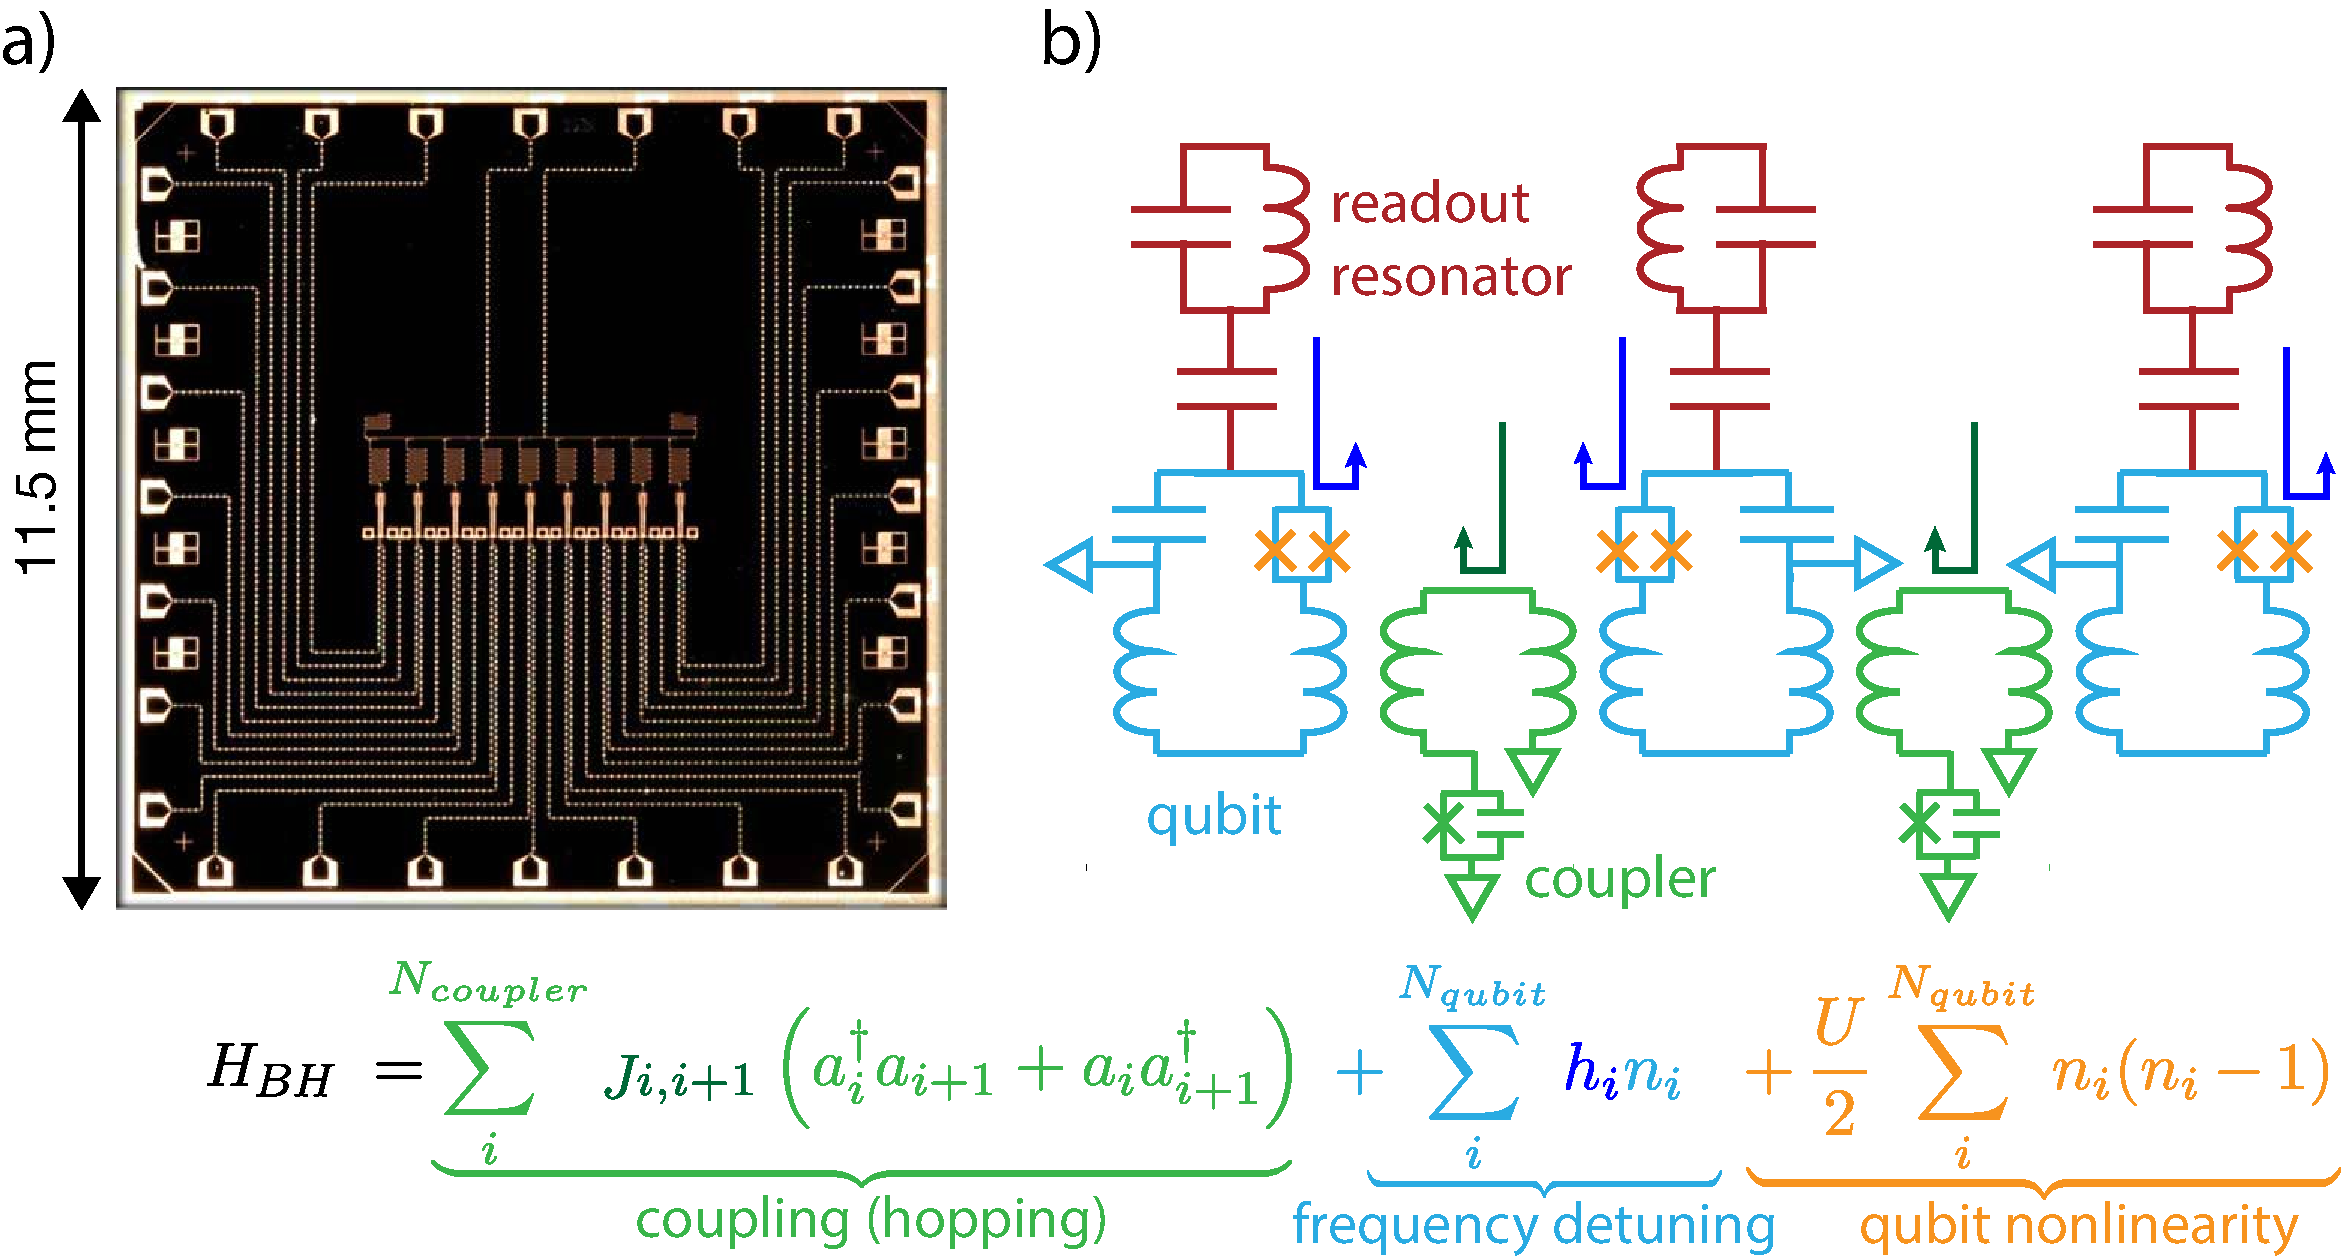
\includegraphics[width=0.80\textwidth, keepaspectratio]{./PDF/fs1_190916_1029a.pdf}
\caption{\textbf{The 9 qubit linear chain device.} This device was used in Figs.\,2-4 of the main text.
\textbf{(a)} Optical micrograph of the $9$ qubit linear-chain device.
\textbf{(b)} Circuit diagram for a three qubit subsection of the device.}
\end{figure}

\subsection{Single qubit gate error rate}
\begin{figure}
\centering
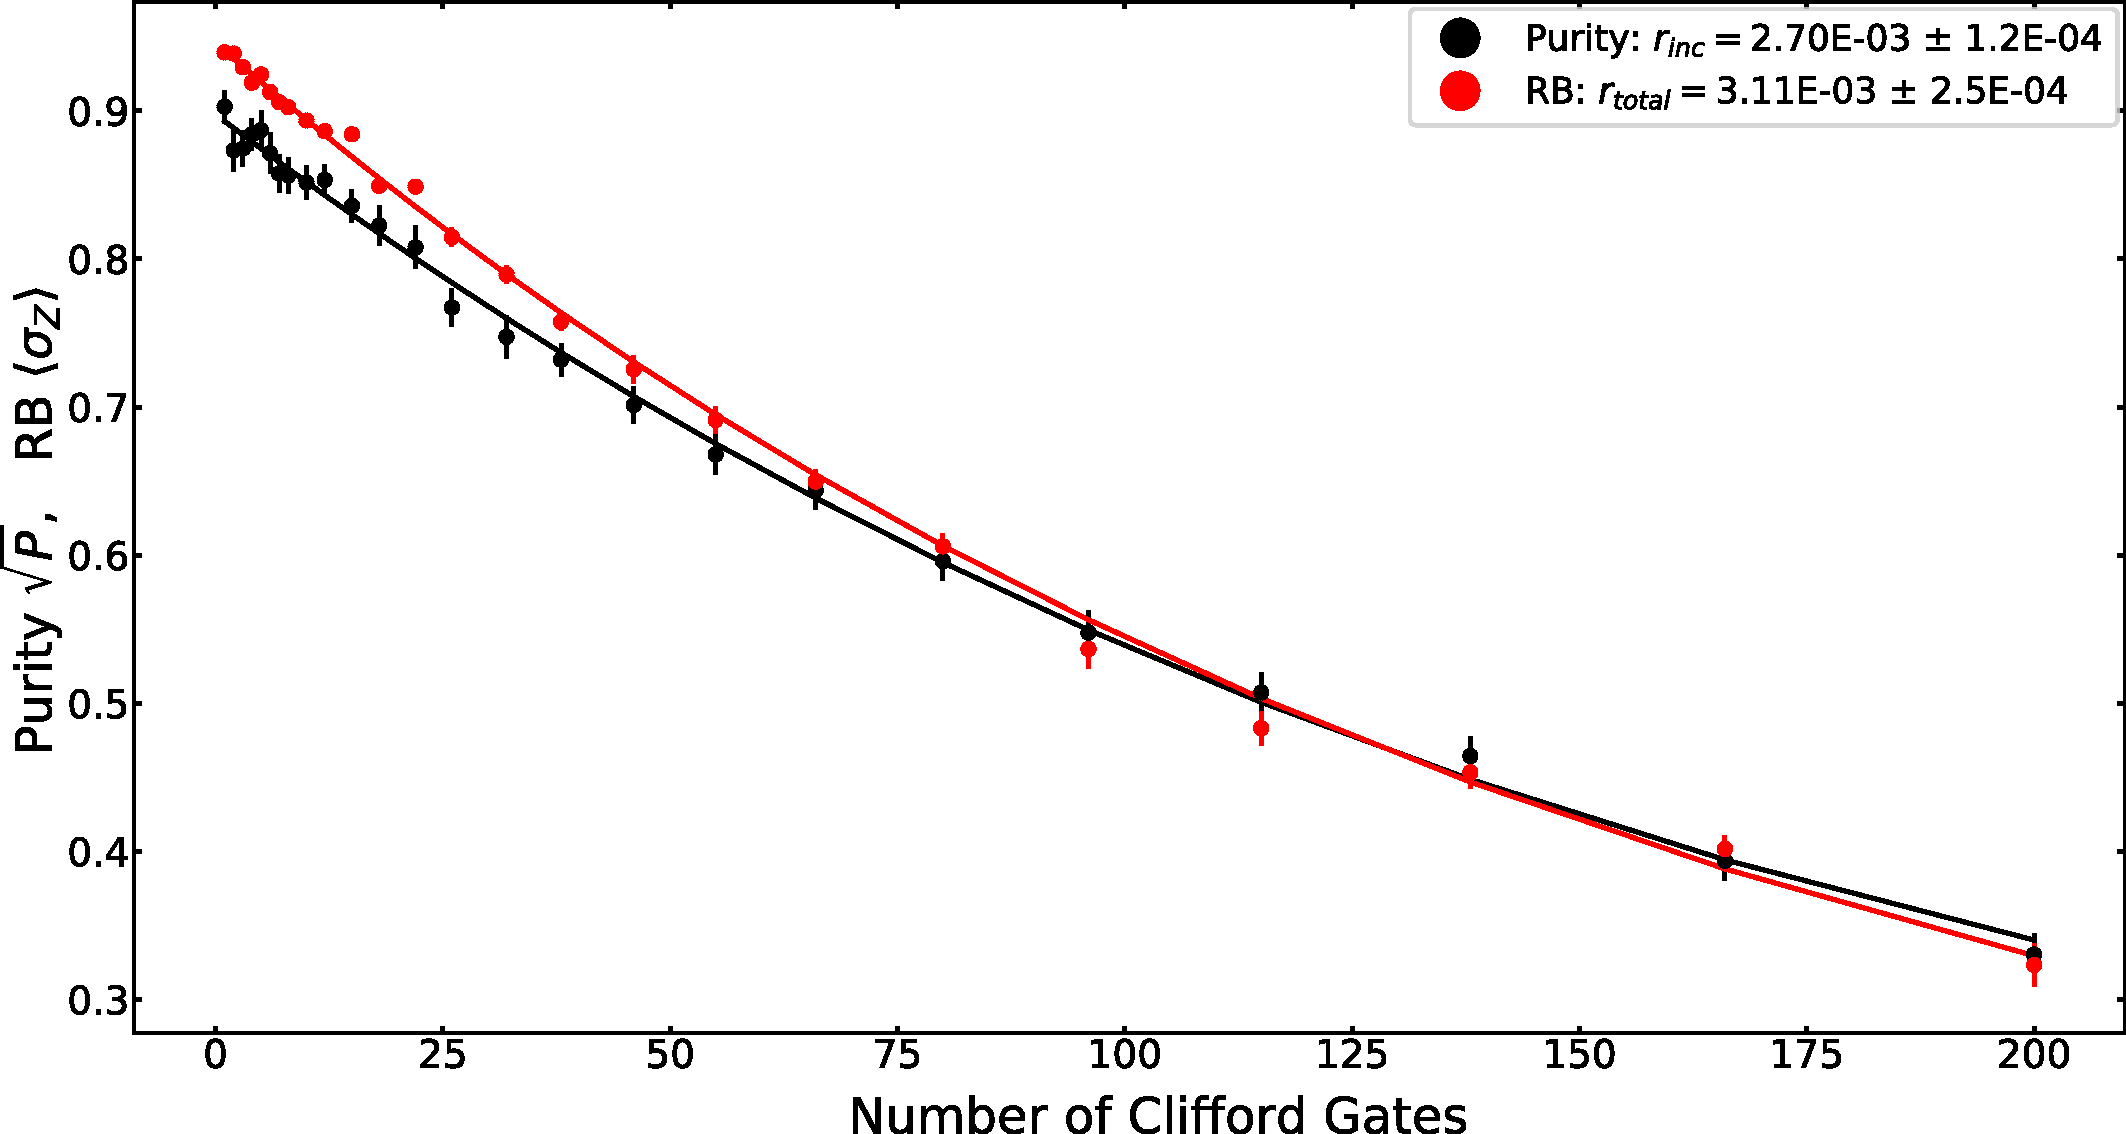
\includegraphics[width=140mm, keepaspectratio]{./PDF/RB_supp_190530_1105a.pdf}
\caption{\textbf{Single qubit gate performance.}  Clifford based randomized benchmarking (RB), shown in red, characterizes the total error rate per Clifford.  Purity benchmarking, shown in black, characterizes the total incoherent error rate per Clifford.}
\end{figure}
We use Clifford based randomized benchmarking (RB) and purity benchmarking to quantify the total error rate and the error rate due to decoherence per Clifford for the single qubit gates in our algorithm.
The data shown in Fig.\,S2 is for a typical qubit.  The total and incoherent error rates per Clifford are extracted to be $3.1 \times 10^{-3}$ and $2.7 \times 10^{-3}$.
Since there are relatively few single qubit gates in our analog algorithms this is not a significant source of error.

\subsection{Manybody Hamiltonian benchmarking}
\begin{figure}
    \centering
    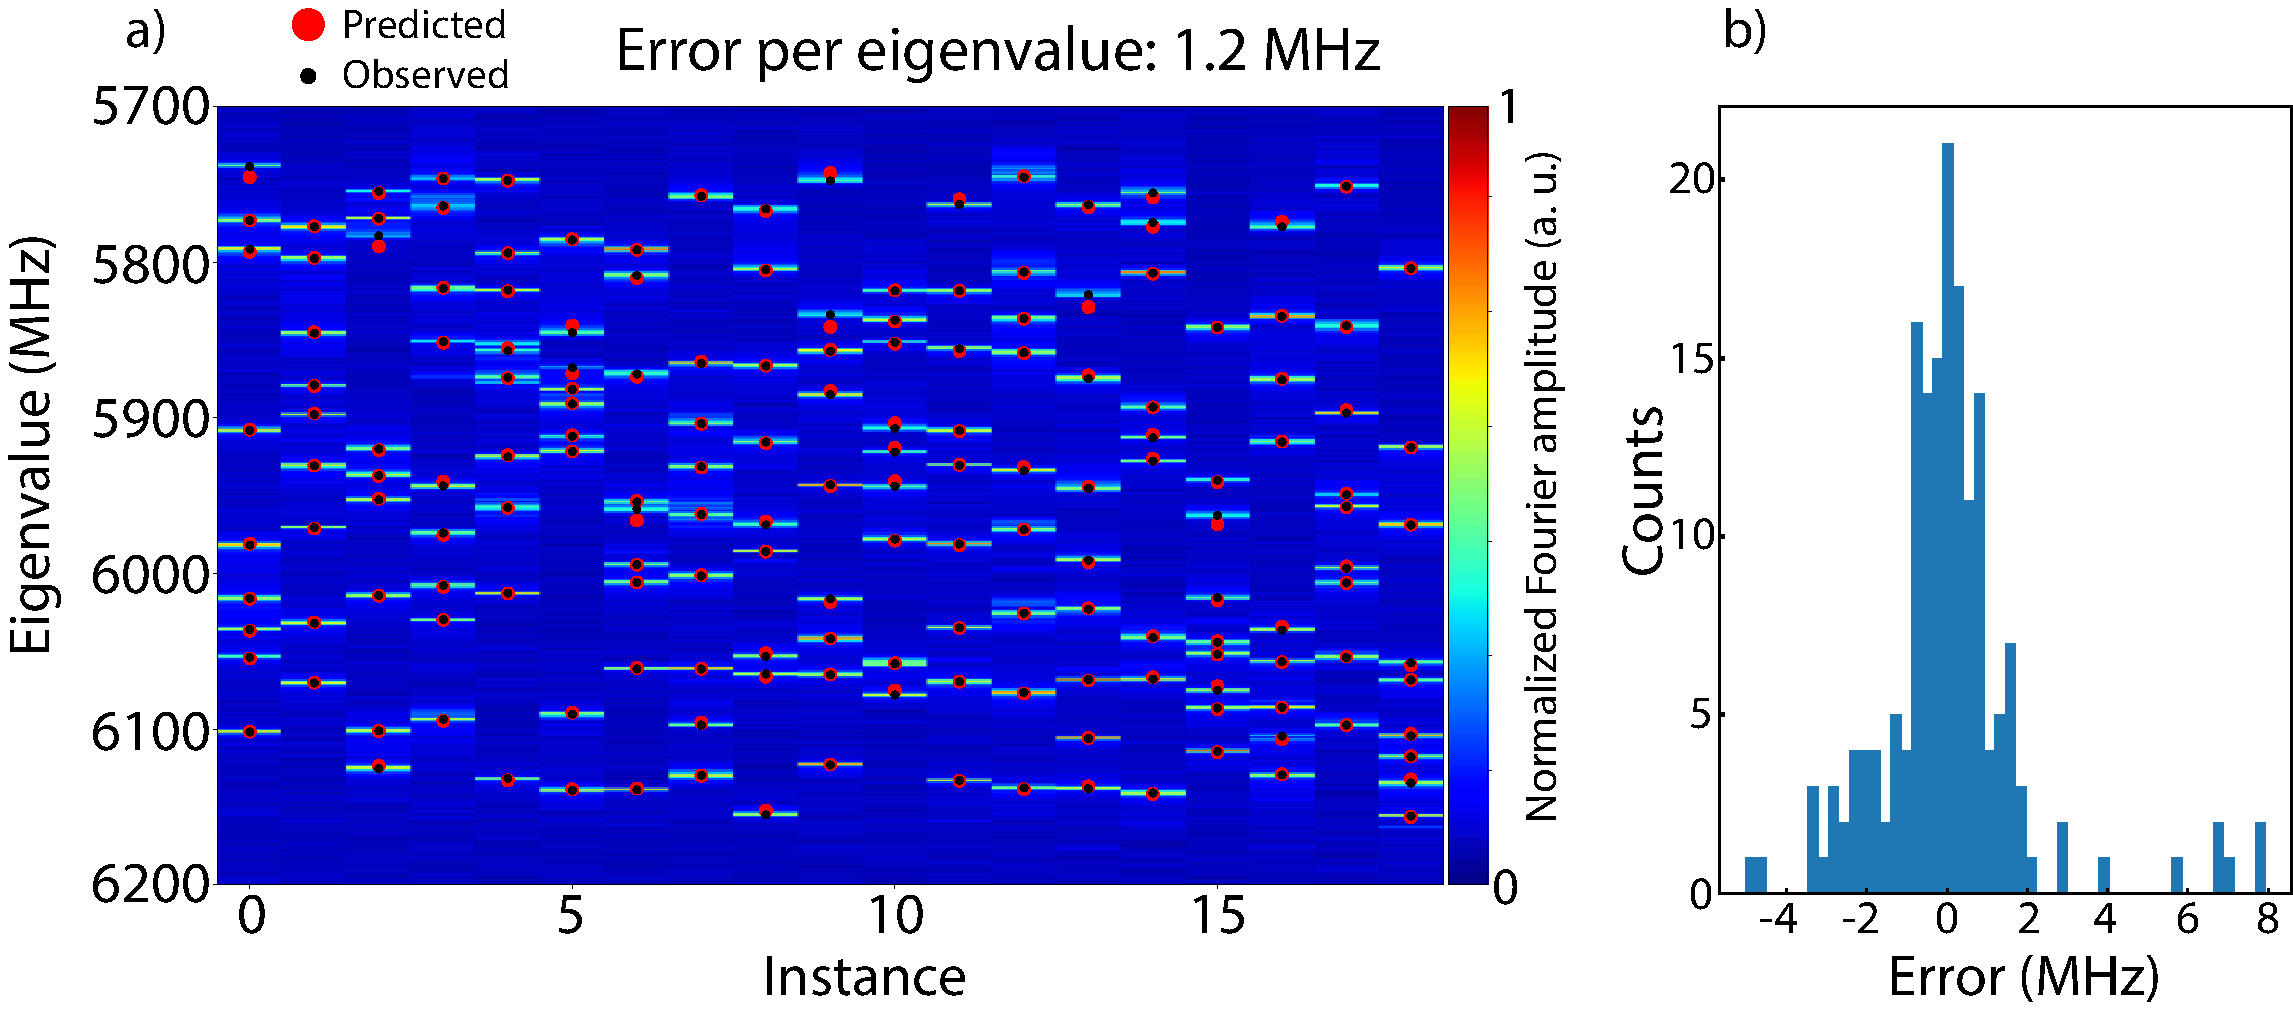
\includegraphics[width=0.9\textwidth, keepaspectratio]{./PDF/random_hamiltonian_calibration_data_190508_549p.pdf}
    \caption{\textbf{Many-body Ramsey calibration data for 9 qubit randomly generated Hamiltonians.}
    \textbf{(a)} Fourier data for 18 instances of randomly generated Hamiltonians overlayed with the control model predictions of the eigenvalues.
    \textbf{(b)} A histogram of the difference between the control model predicted eigenvalues and the experimentally observed peaks.
    }\end{figure}
    In order to benchmark our ability to set multi-qubit time-independent Hamiltonians we compare the eigenvalues predicted by our control model with those observed by using the manybody Ramsey spectroscopy technique \autocite{Roushan2018}.
    We prepare a qubit in the superposition state
    $\ket{\psi_0} = \left( \frac{\ket{0} + \ket{1} }{\sqrt{2}} \right) \otimes \ket{ \text{0, ..., 0} }_{\text{Other}}$,
    evolve the system under a $9$ qubit time-independent Hamiltonian, and observe $\langle \sigma^x + i \sigma^y \rangle$ of the initialized qubit vs evolution time.
    The eigenvalue spectrum can then be recovered by Fourier transforming this time-series.
    This procedure is repeated for each of the qubits in our system and a composite spectrum is assembled from these measurements.
We then compare the eigenvalues predicted by the parameterized circuit model and with those extracted experimentally.  Example calibration data for the 9 qubit linear chain geometry is shown is Fig.\,S3.
    %\endgraf
    %\hspace{\parindent}

    To make a stressful test and benchmark our control model over a wide parameter space we perform manybody Ramsey spectroscopy over several instances of randomly generated Hamiltonians.
    In the 9 qubit data shown here, the coefficients of our target Bose-Hubbard Hamiltonian were taken to be independent random variables with $J_{ij}\, \in[0, 45] \text{MHz}$ and $h_{i} \in[-200, 200] \, \text{MHz}$.
    In Fig.\,S3\,(a) the 2D color map shows the composite spectra for these instances.  The 2D plot is overlayed with the eigenvalue predictions from the control model (red circles) and the detected peak locations (black circles).
    In (b) we report the distribution of errors obtained from the difference of the predicted and observed eigenvalues for each instance.
    The average error per eigenvalue for these Hamiltonian instances is $1.2 \, \text{MHz}$.

\section{Transport measurements, Figs.\,S4-S6}
\subsection{Transport measurement instances}
\begin{figure}[h!]
    \centering
    %\includegraphics[width=0.8\textwidth, keepaspectratio]{./PDF/transport_instances_190531_1214p.pdf}
    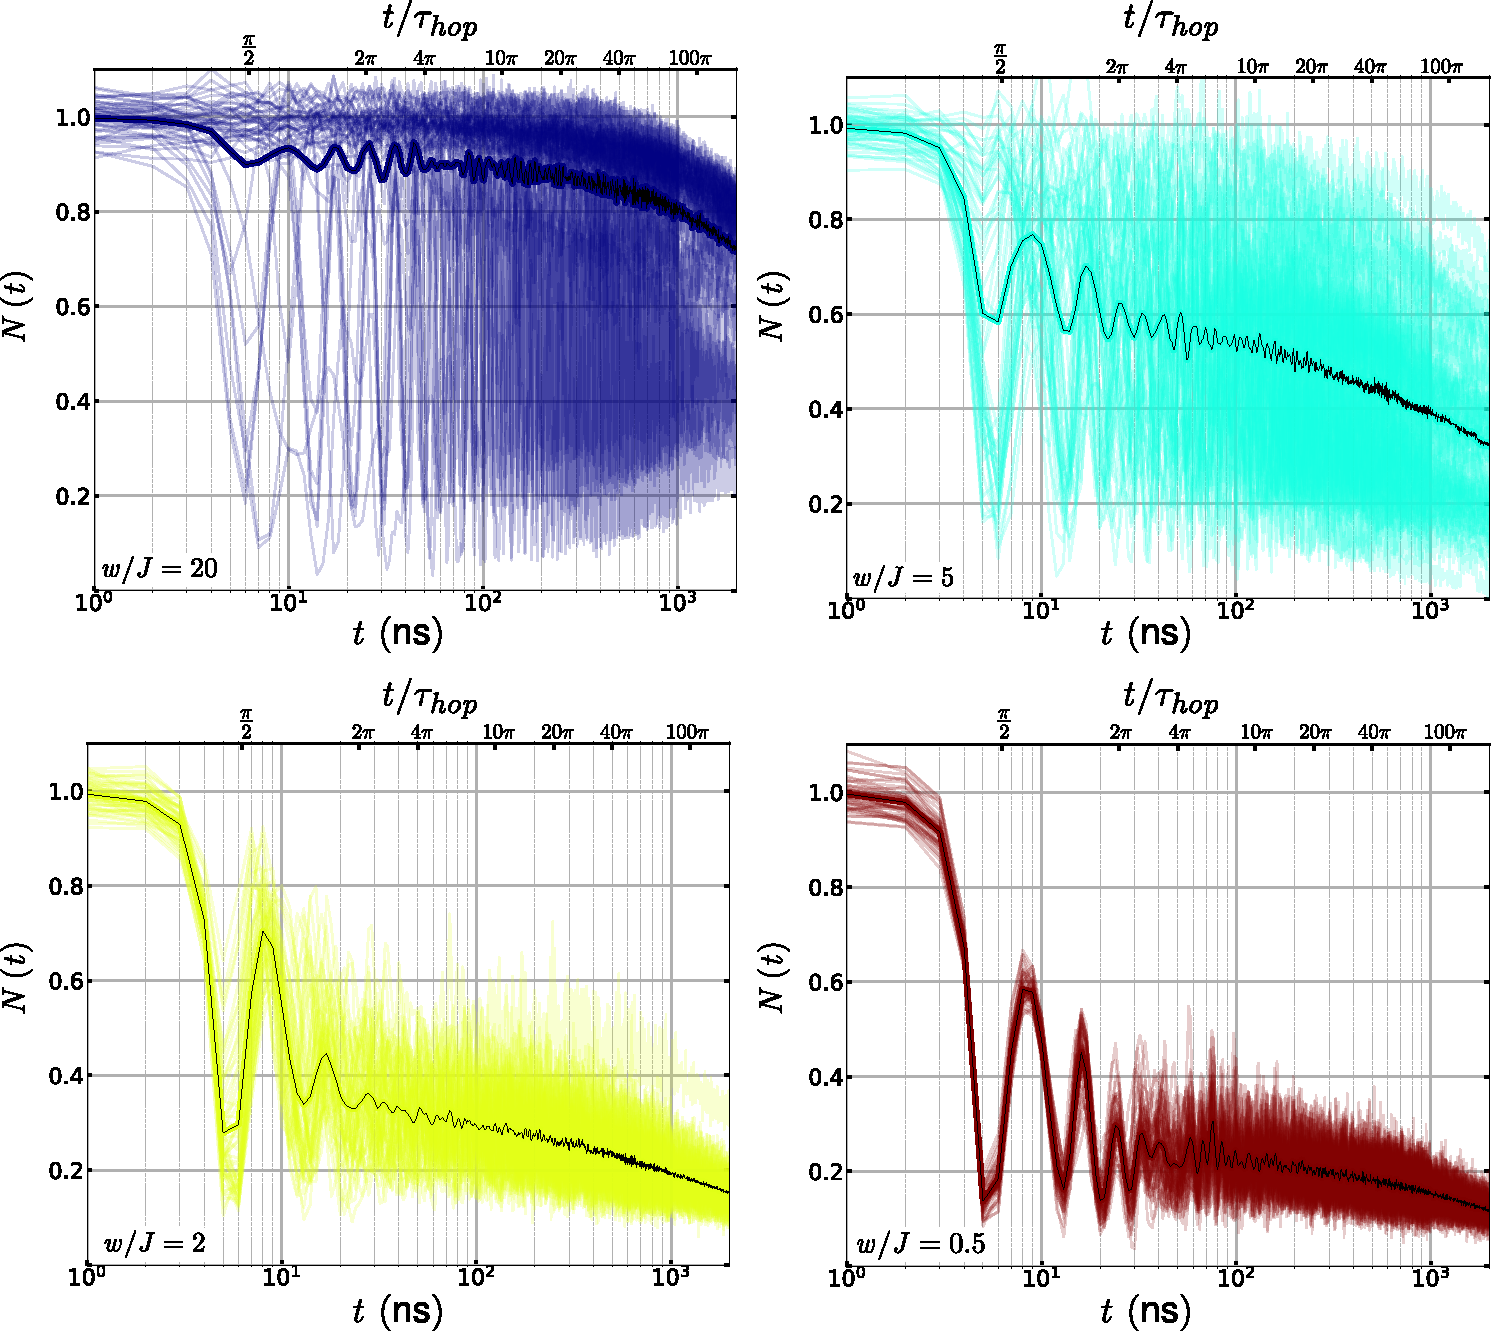
\includegraphics[width=0.8\textwidth, keepaspectratio]{./PDF/fs4_190625_150p.pdf}
    \caption{\textbf{Transport measurement instances.}
    Instances of $N \left( t \right)$ for the transport protocol of main text Fig.\,2 prior to disorder averaging.  Data shown here is for $J=40 \, \text{MHz}$ and $n_{ph}=2$.
    }
    \end{figure}

In Fig.\,S4 we show data from the transport measurements before disorder averaging.  The data shown is for $n_{ph}=2$ and selected values of disorder parameter $w$ for $J = 40 \, \text{MHz}$.
The disorder averaged data (black lines) is contained in Fig.\,2\,(a) of the main text, and the histograms in Fig.\,2\,(b) of the main text are time slices of this data at $100 \, \text{ns}$.
The spread in values at short time is primarily due to readout error, as state preparation error is small.

\subsection{Decoherence effects}
\begin{figure}[h]
\label{decoherence_effects}
\centering
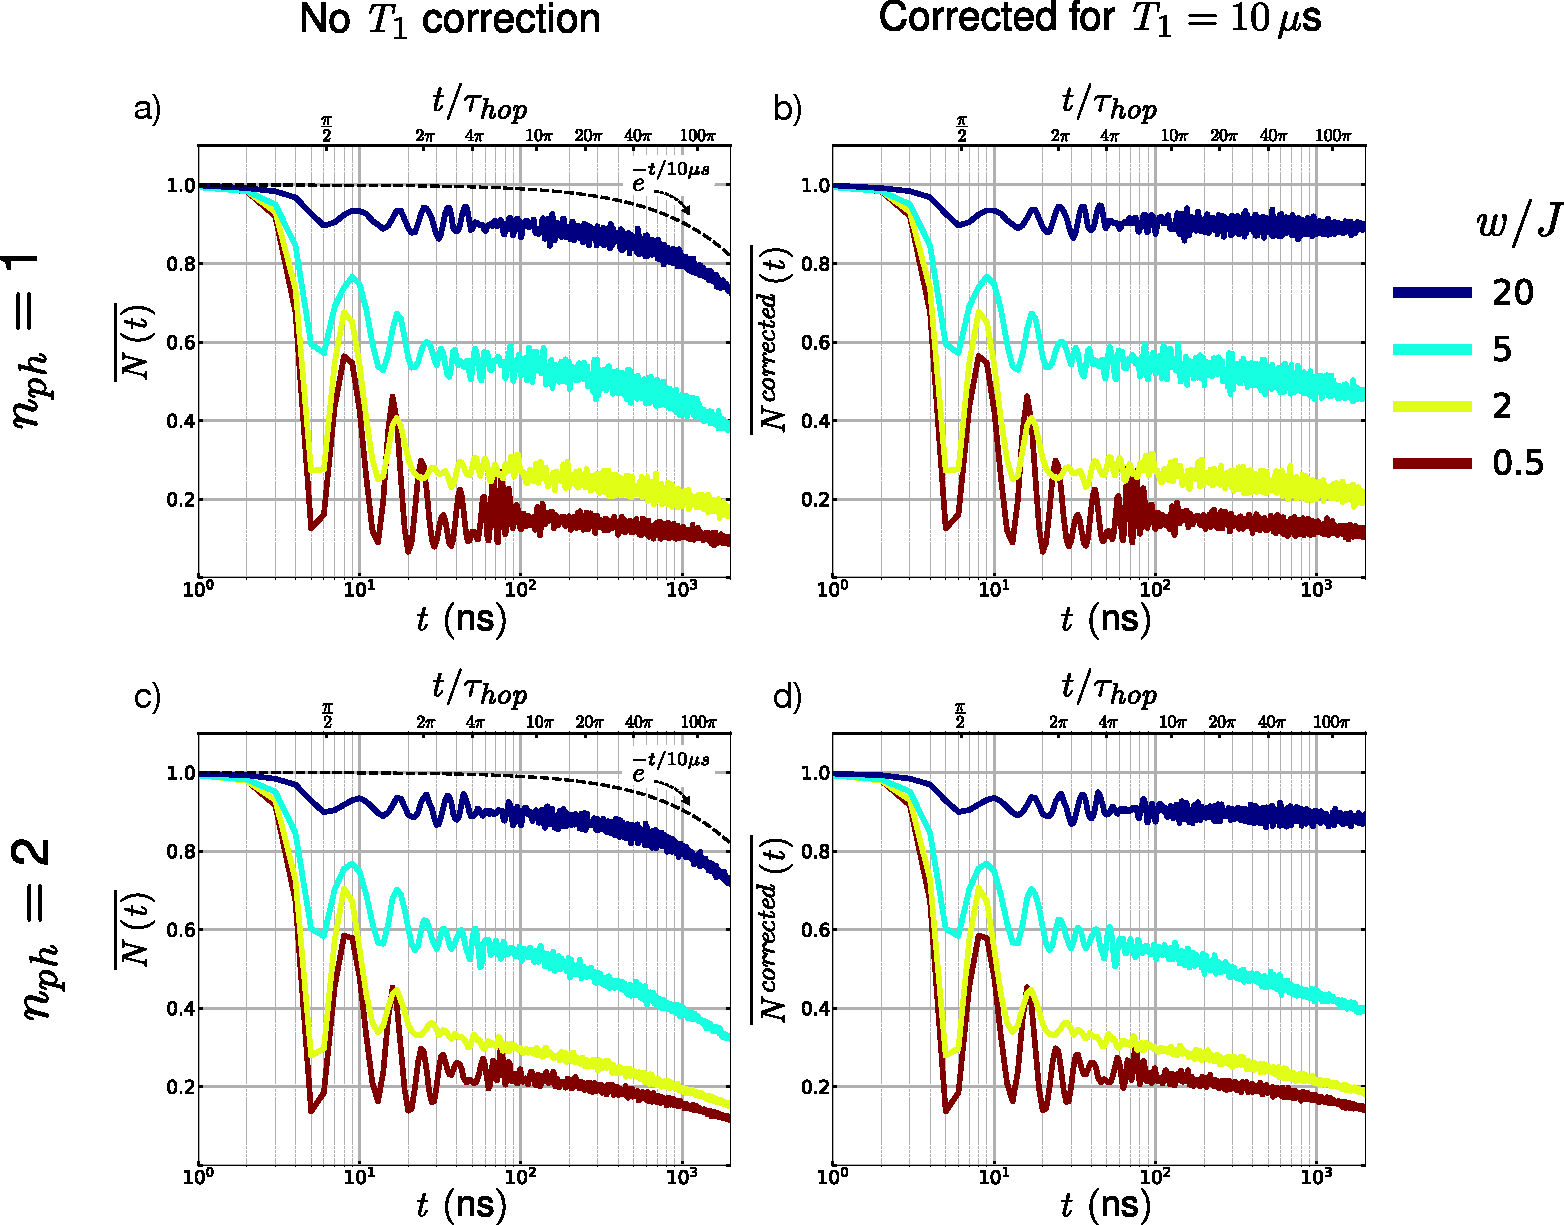
\includegraphics[width=170mm, keepaspectratio]{./PDF/fs5_190919_1208p.pdf}%{./PDF/fig_sup_coherence_effects_190531_356p.pdf}
\caption{\textbf{Transport Measurements:  Decoherence Effects.}
\textbf{(a)} The raw disorder averaged transport data for $n_{ph}=1$
\textbf{(b)} The data from (a) corrected for a simple energy relaxation model $\overline{N^{corrected} \left( t \right)} = \overline{N \left( t \right)} / e^{\left( -t/10 \mu s \right) }$.
\textbf{(c)} The raw disorder averaged transport data for $n_{ph}=2$.
\textbf{(d)} The disorder averaged transport data with $T_{1}$ correction.
}\end{figure}
In the main text we report on short-time dynamics $t\lesssim 100 \, \text{ns}$, before our system is dominated by decoherence.
In reality, our $9$ qubit chain is an open system, subject to both relaxation and dephasing because of its coupling to the environment.
The characteristic relaxation time $T_1$ is $\sim 10 \mu$s and the characteristic dephasing time is a few $\mu$s.
In Fig.\,S4 we provide additional data as an estimate of the importance of these open system effects.
In panel (a) we show the disorder averaged population vs time data for $n_{ph}=1$.
In panel (b) we show the population vs time data for $n_{ph}=1$ after correcting for relaxation (photon loss) using a simple single qubit $T_1$ model
$\overline{N^{corrected} \left( t \right)} = \overline{N \left( t \right)} / e^{\left( -t/10 \mu s \right) }$.
%
At high disorder, where the localization length is shorter than one lattice site,
single qubit $T_1$ (photon loss to the environment) is the dominant mechanism by which a photon leaves the observation site and this correction works well,
as indicated by the fact that the population has taken a stationary value.
%
At low disorder, in the diffusive regime, the excitations are able to distribute themselves evenly across the chain and we expect the $T_1$ correction to work well in this case as well.
Referring to Fig.\,2\,(c) of the main text we see that at $100 \, \text{ns}$ in the diffusive regime at low disorder we measure the thermal expectation values.
This indicates clearly that relaxation effects are not significant in the first $100 \, \text{ns}$.
And that any apparent loss is due to transport within the $9$ qubit chain and not photon loss.
%
For intermediate disorders there appears to be additional photon loss since the onsite population declines. However, the decrease in observed population at the observation site is attributed to dephasing assisted delocalization. \autocite{Znidaric2015, Levi2016, Fischer2016, Luschen2017, vanNieuwenburg2017}

When the LIOM extends over multiple lattice sites, dephasing between the sites breaks down the localized wave-packet by destroying the quantum interference pattern that causes the localization.
This breakdown of coherence between different parts of the wave packet enables transport of the excitation across the $9$ qubit chain.
Crucially, we note that neither $T_1$ relaxation nor dephasing between the lattice sites significantly influence the dynamics at higher disorders or short times.
This feature is captured in the main text Fig.\,4\,(b) where we note that $\overline{ \langle \sigma^{z} \rangle }$ is nearly constant between $10 \, \text{ns}$ and $100 \, \text{ns}$.
In Fig.\,S5\,(c) and (d) we show the raw and $T_1$ corrected data for $n_{ph}=2$.

\subsection{Two state occupation}
\begin{figure}[tbh]
    \centering
    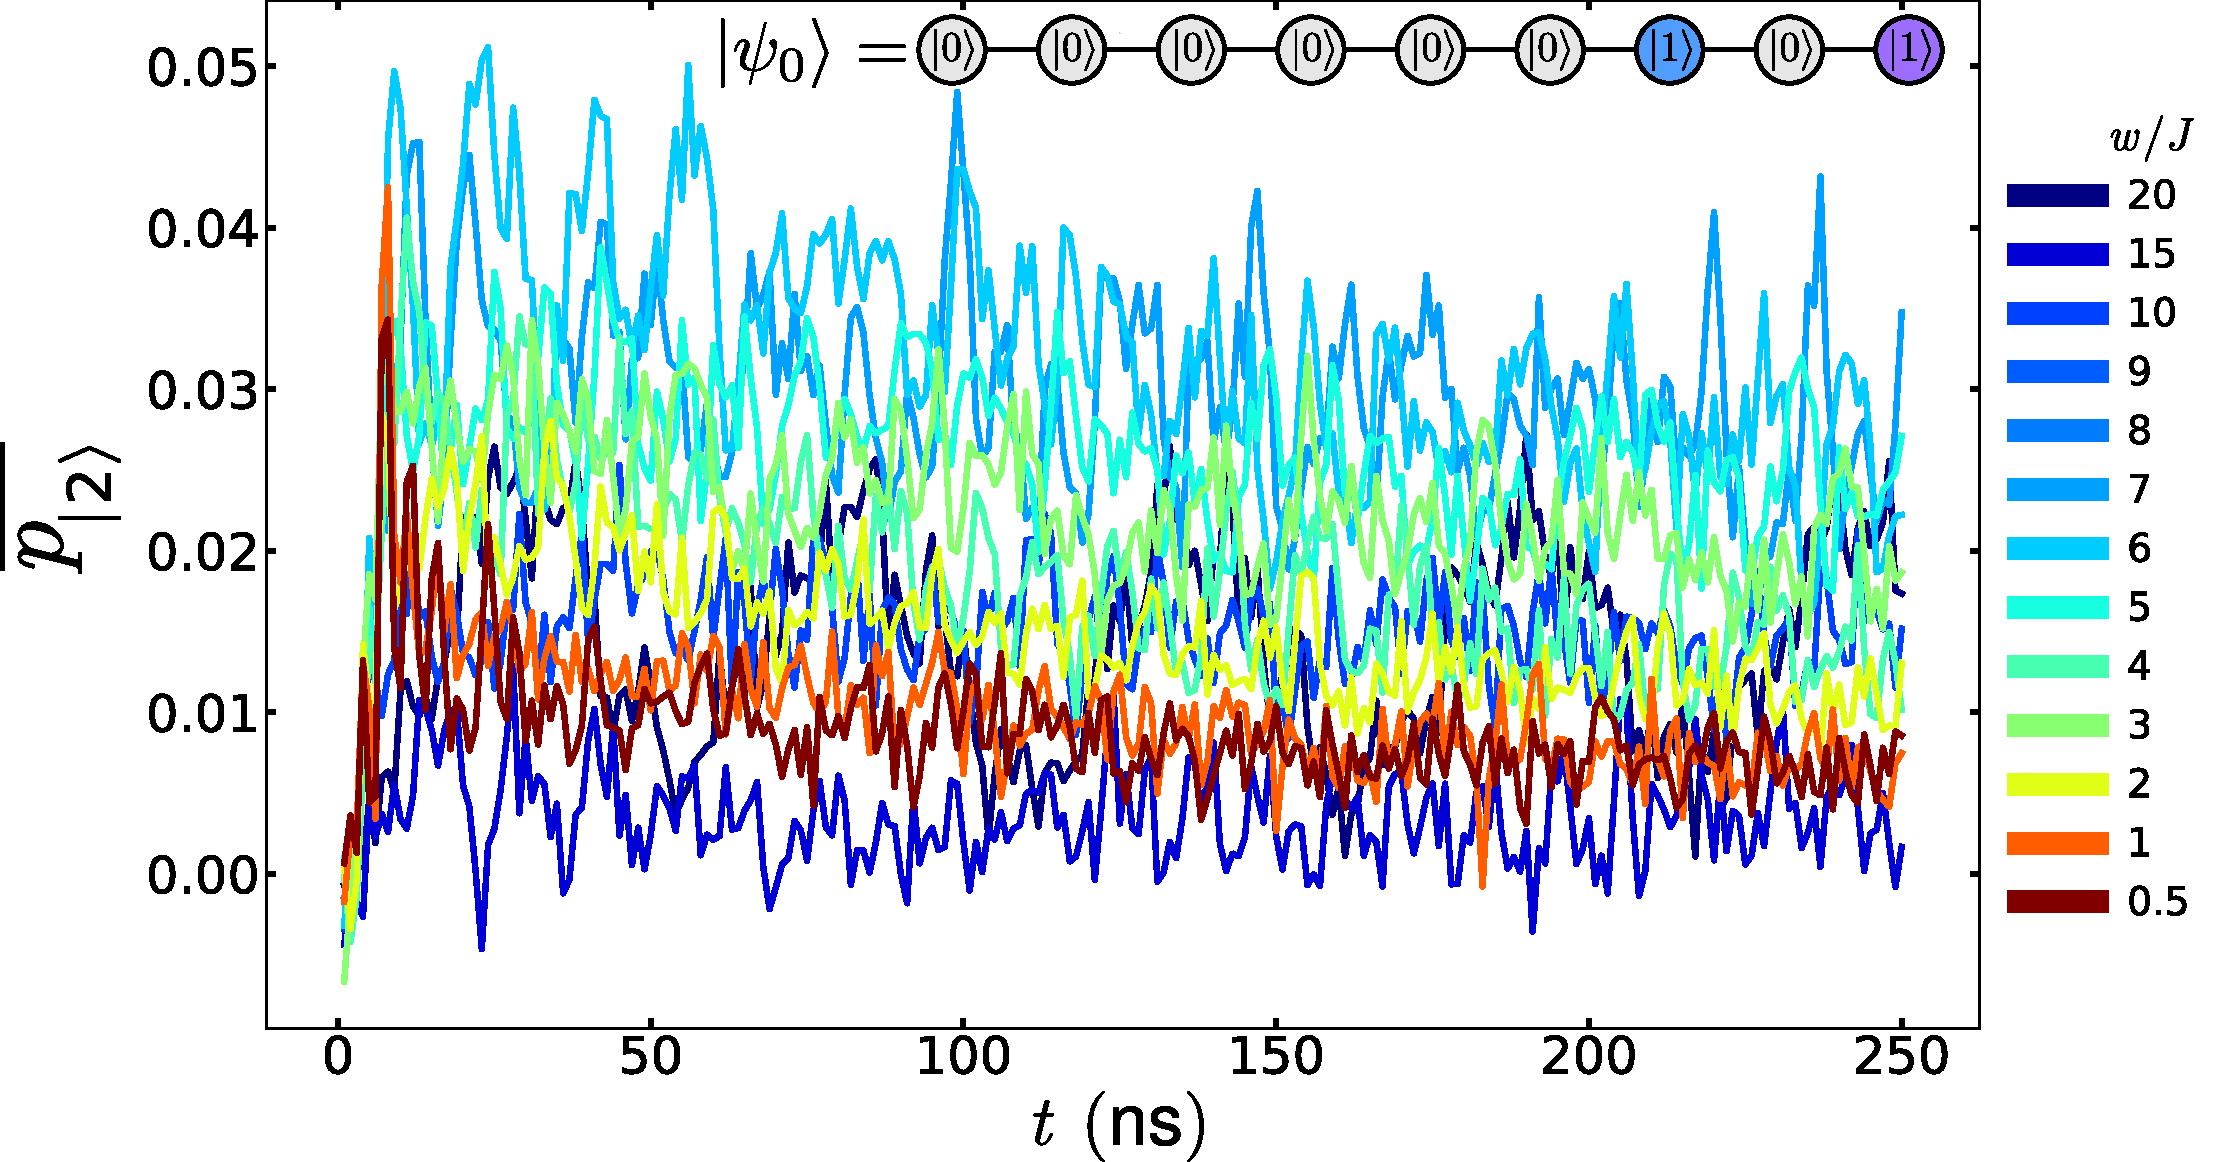
\includegraphics[width=150mm, keepaspectratio]{./PDF/fs6_190919_1238p.pdf}
    \caption{\textbf{Transport Measurements:  Two state occupation.}
    }\end{figure}
    A critical feature of our system is that multiple excitations in the system may interact via the Hubbard interaction.
    The form of this interaction
    $H_{int} = \frac{U}{2}\sum\limits_{n=1}^{n_{Q}} \,a^{\dagger}_{n}a_n(a^{\dagger}_{n}a_n-1)$
    indicates that it is only activated when there are multiple excitations on the same lattice site.
    Thus the interaction effects that we report in the main text require occupation of the higher levels of our Bose-Hubbard lattice.
    In Fig.\,S6 we report the $\ket{2}$ population vs time for a system initially in the state $\ket{\psi_0}=\ket{000000101}$ and observed on the right-most qubit.
    We find that the $\ket{2}$ state population is typically at the 2 \% level,
    achieves its maximum value early in the evolution, and does not progressively grow larger with time.

%%%%%%%%%%%%%%%%  From Michael and Annabelle email 190508
\section{Interferometric protocols, Figs.\,S7-S10}
In order to gain some insights about the echo sequences, we first consider the case of very strong disorder, where the local integrals of motion (LIOMs) $\tau_i^z$ are close to the physical spins $S_i^z$ (represented by the two lowest energy levels of a qubit), and assume that we directly manipulate LIOMs. First, we will consider the spin echo sequence illustrated graphically in Fig.\,S7~\cite{KnapPRL2014}.  Assuming we start from the vacuum state $\left|\psi_0\right> = \left| 0 \right>\otimes \ket{\{\tau_j\}} $, we initiate the dynamics by applying a $\pi/2$ pulse:
\begin{equation}
\ket{\psi} =\frac{1}{\sqrt{2}} (\ket{0} + i \ket{1}) \otimes \ket{\{\tau_j\}}
\end{equation}
When the system evolves for times $t/2$, the spin at site $i$ experiences an effective magnetic field, that depends on the states of the other LIOMs, see Eq. (2) in the main text,
\begin{equation}
\label{field}
\Delta_i = \tilde{h}_i  + \sum_j J_{ij} \tau_j^z + \sum_{j,k} J_{ijk}  \tau_j^z \tau_k^z + \ldots.
\end{equation}
\subsection{Echo pulse sequences}
\begin{figure}[h]
\centering
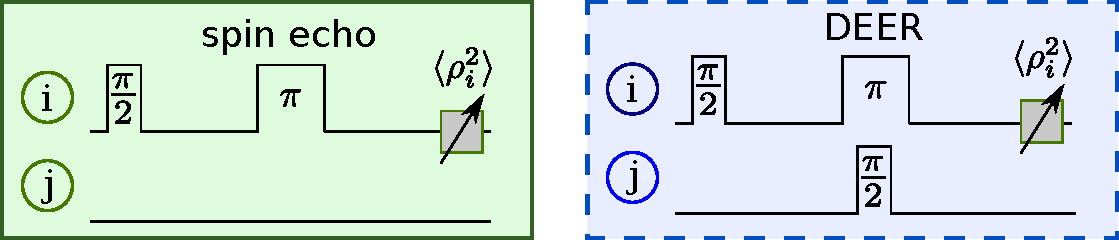
\includegraphics[width=.6\columnwidth]{./PDF/schem2}
\caption{\textbf{Pulse sequence schematics for spin and DEER echo.}  DEER echo differs from spin echo by the addition of a remote $\pi / 2$ pulse simultaneous with the spin echo $\pi$ pulse between the free precession intervals.}
\label{fig:4}
\end{figure}
The $\pi$ rotation halfway through the spin-echo sequence then inverts the effective magnetic field $\Delta_i \to -\Delta_i$ which is precisely canceled after another time evolution for $t/2$. At the end of the protocol we measure the purity, which is advantageous over measuring a single spin component, because it is less prone to running field gradients and external perturbations. For the spin-echo sequence on the LIOMs we find a perfect purity of one.
In a true measurement on our device the echo is performed on the physical spins, which possess a finite operator overlap with the LIOMs which is less than one. This leads to a spin echo signal that saturates to a finite value that decreases with decreasing disorder strength~\cite{KnapPRL2014}.

In the DEER echo sequence we similarly perform a spin echo measurement on site $i$ as before, However, half-way through the time evolution we modify a second part of the system, say site $j$ by applying a $\pi/2$ pulse, see
Fig.\,S7. The effective magnetic field for the backward evolution $\tilde \Delta_i$, deviates from the field $\Delta_i$ of the forward evolution in all the terms containing $\tau_j^z$.
In summary, the state after the second time evolution is therefore
\begin{equation}
\begin{aligned}
\ket{\psi_{D}(t)} = \frac{1}{2} [& \ket{1}\otimes\ket{...0_j...} + e^{i (\Delta_i-\tilde{\Delta}_i) t - i\Delta_j t} \ket{1}\otimes \ket{...1_j...} - \\
&\ket{0}\otimes\ket{...0_j...}- e^{-i (\Delta_i-\tilde{\Delta}_i) t - i \Delta_j t} \ket{0}\otimes \ket{...1_j...}
]
\label{eq:deer_finaltime}
\end{aligned}
\end{equation}
and the measurement of the purity then yields
\begin{equation}
\tr \left(\rho^2\right) = \cos^2\left[\left(\Delta_i-\tilde{\Delta}_i\right) t\right].
\end{equation}

Due to the interaction between the $\tau$ bits at site i and j, the phases do not cancel anymore and the signal decays. The difference between spin and DEER echo is thus a pure interaction effect which would not appear in the noninteracting localized phase. The advantage of performing a differential measurement of the two echo protocols is that even in the presence of noise, deviations of the two echo signals, demonstrates a clear interaction effect and hence is able to unambiguously measure the interacting character of the LIOMs.
Because these interaction effects are due to the local occupation of higher orbitals we numerically estimate the population of multiply excited states $n_i^{max} = 1,2,3$ during the DEER echo protocol for a evolution time of $t = 63 \, \text{ns}$ in Fig.\,S8.

In the experimental measurement of the purity, local occupations higher than two are not taken into account. This leads to a leakage of the measurement as characterized by the finite value of $\langle \sigma^z_i\rangle$ in Fig. \,3\,(b) of the main text. Moreover, we numerically estimate this effect by resolving the probabilities for maximum local occupations $n_i^{max} = 1,2,3$ during the DEER echo protocol for a evolution time of $t = 63 \, \text{ns}$ in Fig.\,S8.
From that it can be deduced that leakage effects are not severe, and in particular does not change the qualitative difference between the spin echo and DEER echo protocols.
%%%%%%%%%%%%%%%%%%%%%%%%%%%%%%%%%%%%%%%%%%%%%%%%%%%%%
\subsection{Maximum local occupation}
\begin{figure}
\centering
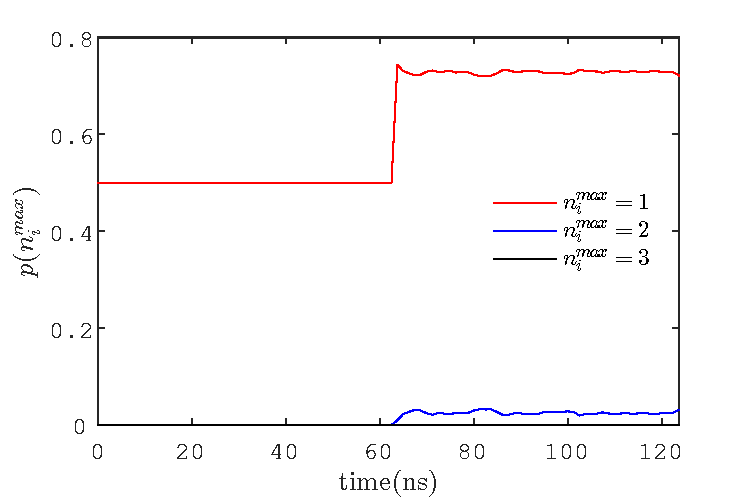
\epsfig{file=./PDF/nimax_L9_N4_nmax3_J04_U16_mu4_tMax125_nReals50_nSReals1.pdf, width=130mm}
\caption{\textbf{Numerical estimate of the occupation of higher transmon levels during the DEER echo protocol.} Calculation shown here for for the one, two, and three excitation states}
\label{figLocalOcc}
\end{figure}
Probability for maximum local occupations of $n_i^{max} = 1,2,3$ during the DEER echo protocol for $L=9$ sites, an evolution time of $T=63$ns, coupling $J=2\pi \cdot 40$MHz, disorder strength $w/J=10$ and interaction $U/J=4$.
%%%%%%%%%%%%%%%%%%%%%%%%%%%%%%%%%%%%%%%%%%%%%%%%%%%%%
%%%%%%%%%%%%%%%%  End From Michael and Annabelle email 190508
%%%%%%%%%%%%%%%%%%%%%%%%
%%%%%%%%%%%%%%%%%%%%%%%%  Discussion of Echo
%%%%%%%%%%%%%%%%%%%%%%%%

\subsection{Comparison with numerics for echo experiments}
\begin{figure}
\centering
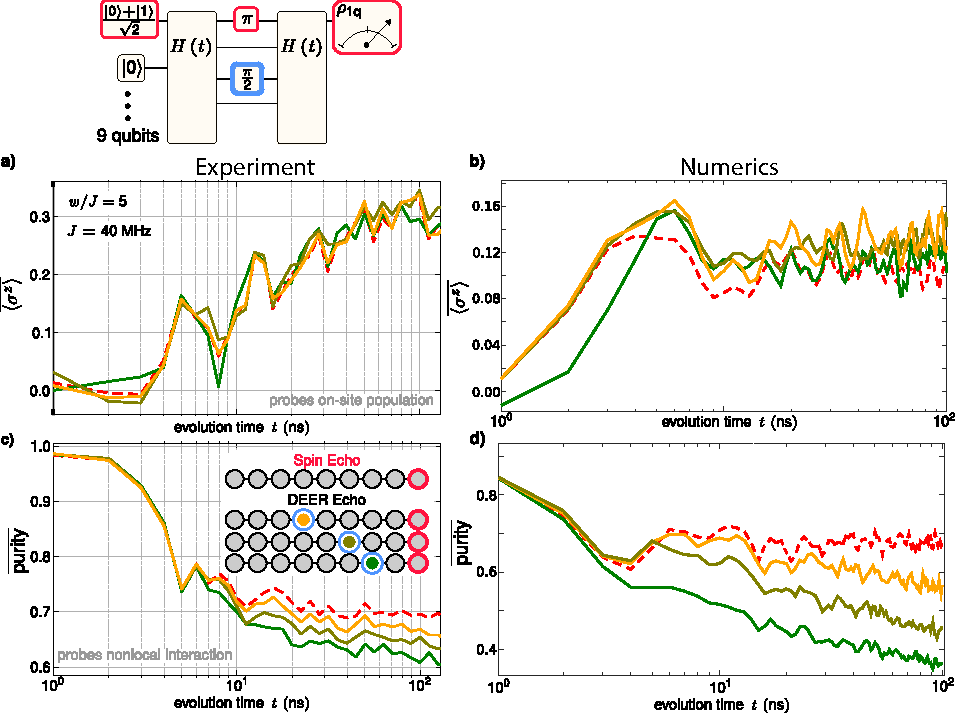
\includegraphics[width=140mm, keepaspectratio]{./PDF/echo_numerics_comparison_190919_944a.pdf}
\caption{\textbf{Comparison with numerics for echo experiments}.
\textbf{(a)} and \textbf{(b)} Disorder averaged expectation value of $\sigma^z$ showing population at the observation site for experimental observations and numerical prediction.
The lack of dependence of $\overline{ \left< \sigma^z \right> }$ on the DEER pulse indicates localization in our system.
\textbf{(c)} and \textbf{(d)} Disorder averaged purity of the reduced single qubit density matrix at the observation site.
The contrast between spin-echo and DEER echo demonstrates that the local phase accumulation is conditional on the remote population.
This is a direct measure of the nonlocal interaction strength.}
\end{figure}

In Fig.\,S9 we compare the data from the interferometric pulse sequences presented in Fig.\,3 of the main text with numeric predictions.  In panels (a) and (b) we compare the onsite population at the spin echo qubit.  Although there is a strong correspondence, we observe greater diffusion off site (larger $\sigma^z)$)  in the experiment than in the numerics.  There is also less contrast in the experiment than in the numerics.  It is likely that these differences are related to the transient pulse response of our system and open systems effects, however further investigation is needed to make a conclusive determination.

\subsection{Extended data}
\begin{figure}
\centering
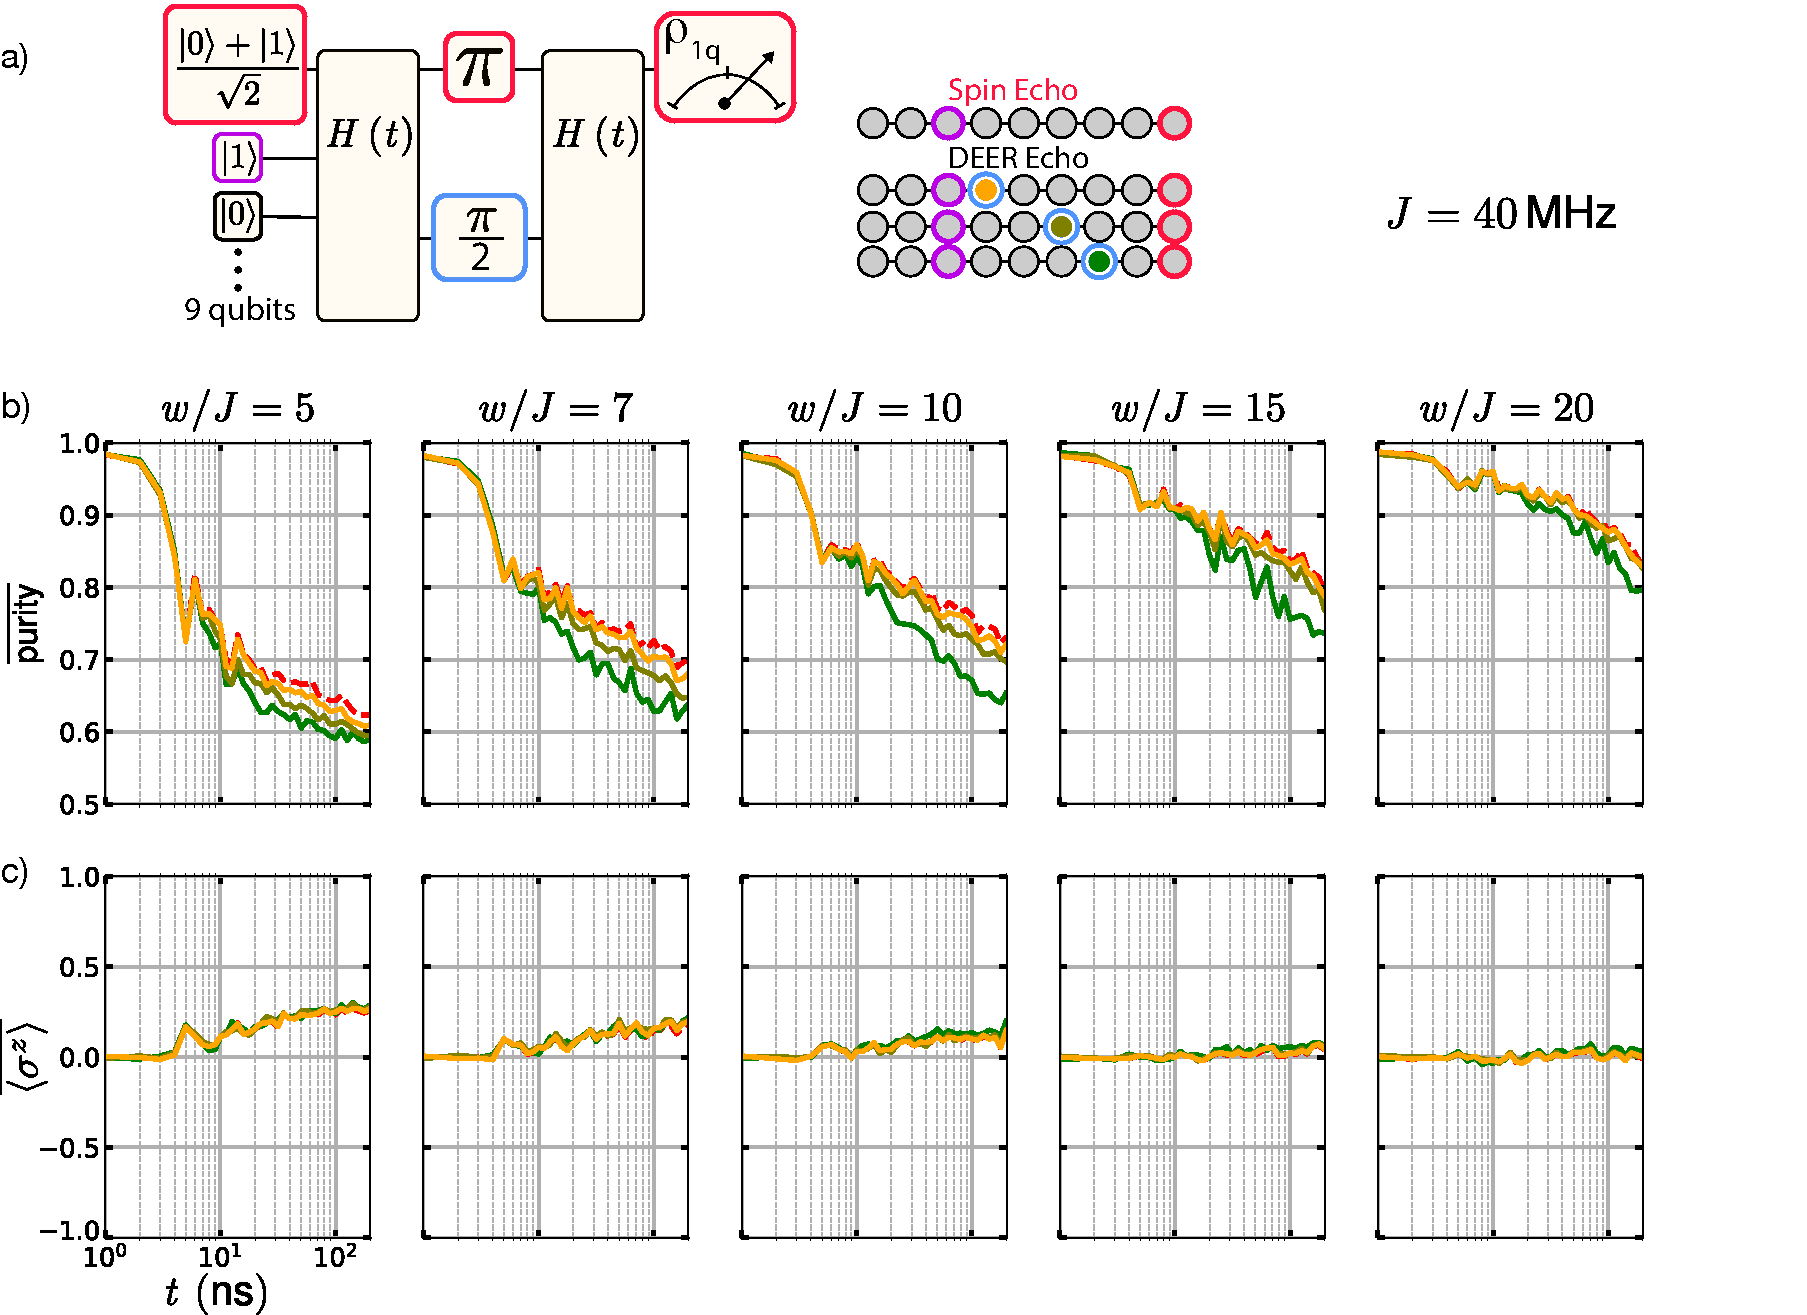
\includegraphics[width=140mm, keepaspectratio]{./PDF/fs9_190919_513p.pdf}%{./PDF/fig_sup_echo_extended_190612_355p.pdf}
\caption{\textbf{Interferometric Protocols:  Extended Data.}
\textbf{(a)} Spin and DEER echo pulse sequences.  We the blue outline indicates the position of the DEER echo pulse, and the position of an additional excitation is indicated in purple.
\textbf{(b)} purity of the single qubit density matrix after the spin echo (dashed red lines) and DEER echo (solid lines) experiments.
\textbf{(c)} $\left< \sigma^z \right>$ monitored over the echo experiments.
}
\label{fig_3}
\end{figure}

In Fig.\,S10 we show extended data for echo sequence measurements for several values of of the disorder parameter $w$ with $J$ held fixed at 40\,MHz.  Compared with Fig.\,3 of the main text, the initial state for these measurements had an additional excitation at the indicated position (purple).  We observe a strong interferometric signature in the purity, indicating nonlocal interaction.  In these measurements $\sigma^z$ does not depend on the position of the echo pulses, indicating localization.

%\textbf{(b)} and \textbf{(c)} are averaged over N instances of disorder.

%\section{Logarithmic growth of entanglement initial state dependence (numerical analysis), Fig.\,S11}
%In the main text we initialize the subsystem qubits into superposition in order to observe the development of entanglement.
%Here we give numerical evidence to support that choice of initial state.
%The growth of entanglement depends strongly on the choice of initial state.
%Intuitively, since the system is localized and on-site population is constant,
%we expect to observe the strongest entanglement growth by preparing the system into a phase sensitive initial state.
%%%\begin{figure}[tbh]
%%%\subsection{Numerical analysis}
%%%\centering
%%%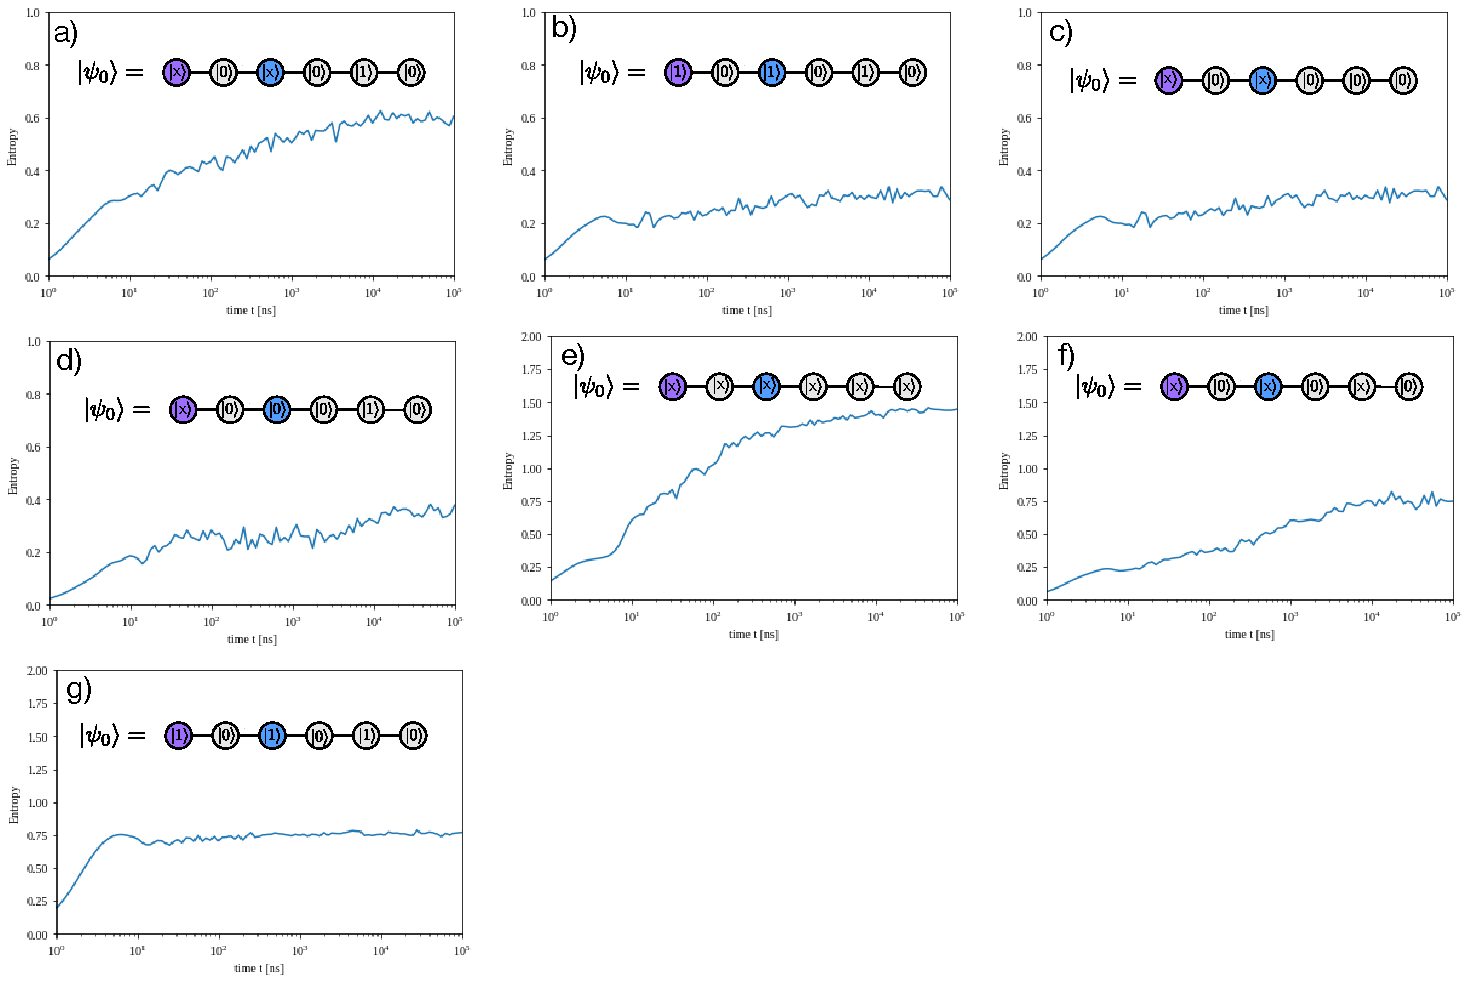
\includegraphics[width=0.8\textwidth, keepaspectratio]{./PDF/log_growth_initial_state_numerics_mk_190612_458p.pdf}
%%%\caption{\textbf{Entanglement growth numerical study.}
%%%\textbf{(a)}, we use an initial state that is analogous to the state chosen in the experimental work in the main text for Figs.\,4\,(b), 5\,(a).
%%%In this case we observe entanglement growth consistent with the experimental observations. There is a sharp increase in entanglement entropy during the first hopping interval, followed by entanglement growth consistent with logarithmic time dependence before saturating at long times.
%%%\textbf{(b)} the system is initialized with excitations rather than superposition states and exhibits extremely weak entanglement growth after the first hopping interval.
%%%This exemplifies the importance of the superposition state initialization in our detector region.
%%%\textbf{(c)} the system is initialized with only the sites in the detection region into a superposition.
%%%In this case there is no excitation on site 3 with which to interact and the entanglement growth and the entanglement growth is much weaker than in (a).
%%%\textbf{(d)} the first qubit is in a superposition state and there is one excitation outside the subsystem. Entanglement growth is reduced compared to (a) because interactions kick in only at exponentially later times giving rise to an intermediate plateau.
%%%\textbf{(e)} all qubits are initialized into superposition states and the system becomes rapidly entangled.
%%%\textbf{(f)} every other qubit is in a superposition state and the system accumulates entanglement continuously, although not as rapidly as in (e) (please note the different y-axis scales).
%%%\textbf{(g)} with every other qubit initialized into an excitation state there is only extremely weak growth of entanglement after the first hopping time scale.}
%%%\label{log_growth_initial_state_numerics}
%%%\end{figure}
%%%On a 6 site chain we perform numeric analysis to show the importance of initial state in the development of entanglement entropy.  We note that there is significant initial state dependence.

%%%%%%%%%%%%%%%%  From Michael and Annabelle email 190508
\section{Entanglement measures}
The distillable entanglement of the two qubit density matrix $E_D(\rho_{2q})$ is lower bounded by the coherent information entropy
\begin{equation}
E_D(\rho_{2q}) \geq S(\rho_{1q}) - S(\rho_{2q}),
\end{equation}
where $\rho_{1q,2q}$ are the reduced density matrices of one of the two qubits and the two qubit subsystem, respectively, and $S(\rho)$ is the von Neumann entanglement entropy.
An upper bound to the distillable entanglement is provided by the logarithmic negativity\autocite{Vidal2002} which is defined as
\begin{equation}
E_N(\rho_2) = \log_2 || \rho_2^{T_A} ||_1.
\end{equation}
Here, $\rho_2^{T_A}$ is the partial transpose of the reduced density matrix with respect to one of the qubits and $|| \cdot ||_1$ denotes the trace norm.

A second operational entanglement measure is the entanglement of formation, which is a measure for the entanglement needed to create a given entangled state.%\autocite{Wootters1998}.
It is defined as
\begin{equation}
E_F(\rho) = \epsilon(\mathcal{C}(\rho))
\end{equation}
with
\begin{equation}
\epsilon(x) = -h_+(x) \log_2 h_+(x) - h_-(x)\log_2 h_-(x)
\end{equation}
where
\begin{equation}
h_{\pm}(x) = -\frac{1}{2} \left(1\pm \sqrt{1-x^2} \right).
\end{equation}
The concurrence $\mathcal{C}(\rho)$ of a mixed state of two qubits is defined as
\begin{equation}
\mathcal{C}(\rho) = \max \left(0,\lambda_1-\lambda_2-\lambda_3-\lambda_4\right),
\end{equation}
where $\lambda_i$ are the eigenvalues of
\begin{equation}
R = \sqrt{\sqrt{\rho}\tilde{\rho}\sqrt{\rho}}
\end{equation}
and
\begin{equation}
\tilde{\rho} = (\sigma_{y}\otimes\sigma_{y})\rho^{*}(\sigma_{y}\otimes\sigma_{y}).
\end{equation}
%%%%%%%%%%%%%%%%  From Michael and Annabelle email 190508
\section{Density matrix evolution numerics comparison, Figs.\,S11 - S15}
\subsection{Comparison with numerics for superposition initial state.}
\begin{figure*}[tbh]
\centering
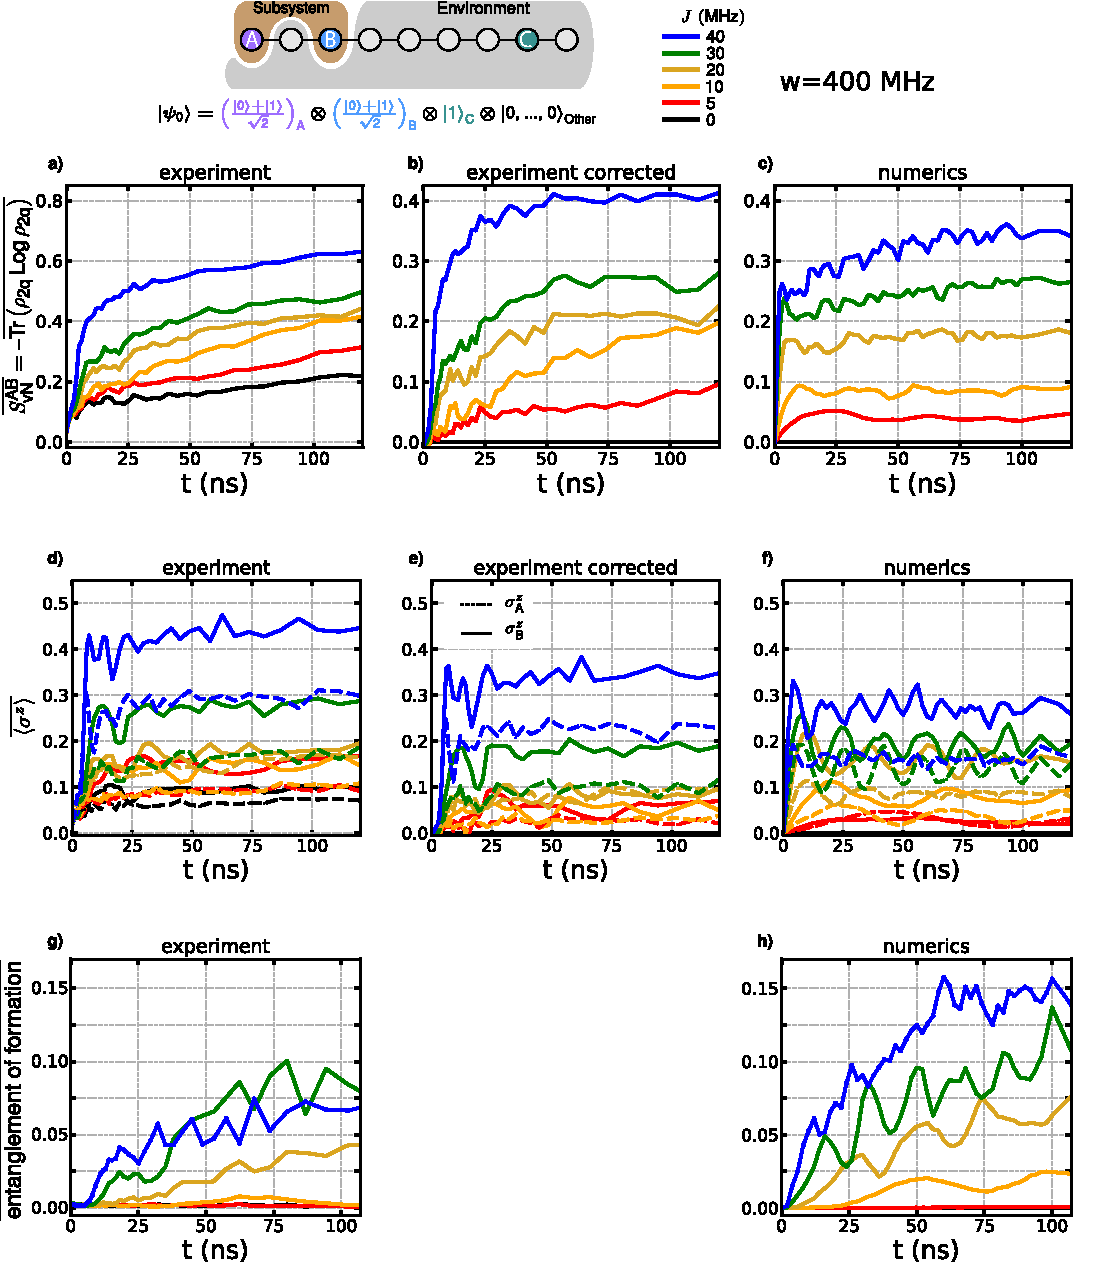
\includegraphics[width=140mm, keepaspectratio]{./PDF/dat_cor_num_superposition_linear.pdf}
\caption{\textbf{Entropy Comparison with Numerics}
\textbf{(a)} Raw experimental observations from the two qubit density matrix measurements.  The $J=0$ data acts as a control experiment.
We attribute entropy accumulation in the control experiment to open system effects
\textbf{(b)} Experimental data after subtracting the baseline entropy measured in the control experiment from each of the data series.
\textbf{(c)} Result of exact diagonalization numerics.
\textbf{(d)} Raw experimental observation of $\sigma^z$, quantifying population.
For the $J=0$ baseline case we attribute the non-zero $\sigma^z$ to state initialization error, and relaxation processes T1.
\textbf{(e)} Experimental data corrected by subtracting the value of $\sigma^z$ in the $J=0$ control experiment from each of the data series.
\textbf{(c)} Prediciton from exact diagonalization numerics.
\textbf{(g)} Entanglement of formation as observed in the experiment.
This is an affirmative observation of quantum correlation between sites A and B which cannot be attributed to open system effects, in contrast to the von Neumann entropy.
The EOF observed in the experiment is slightly damped due to open system effects.}
\end{figure*}

In the main text we observe the entropy accumulation of an x-polarized subsystem in an MBL environment.
The von Neumann entropy represents contributions from entanglement within the 9 qubit system, as well as from open system effects.  In Figs.\,S11-S14 we provide supporting information to assist the reader in estimating the role of open systems effects in our experiment.  We find that a good estimate of the contribution to the von Neumann entropy coming from coupling to the open system is provided by the entropy of the $J=0$ curve.  In the $J=0$ case we do not expect interaction with the environmental qubits and attribute observed entropy in that case to extrinsic dephasing and relaxation processes.

\subsection{Comparison with numerics for bell initial state.}
\begin{figure*}[tbh]
\centering
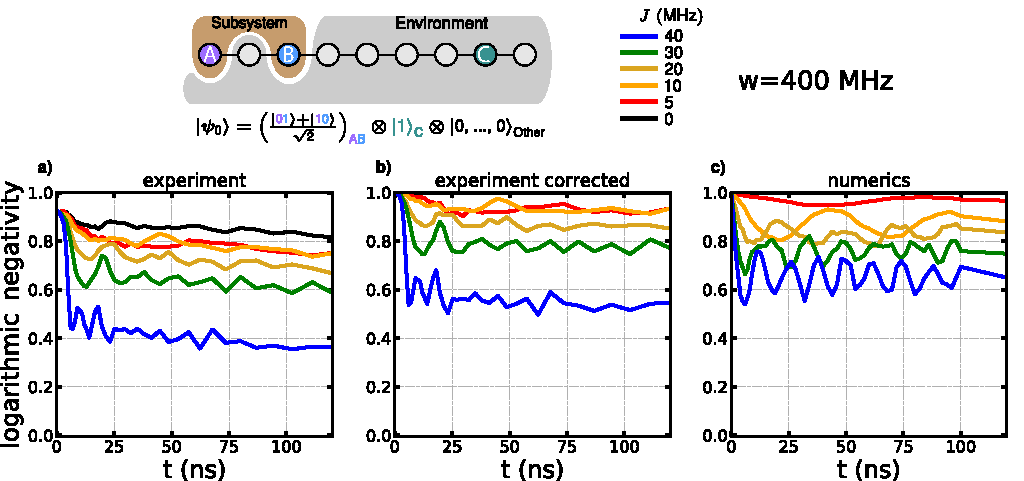
\includegraphics[width=140mm, keepaspectratio]{./PDF/dat_cor_num_bell_linear.pdf}
\caption{\textbf{entropy comparison with numerics}
\textbf{(a)} logarithmic negativity as observed in the experiment.
the black $J=0$ curve is our control experiment, and departure of the logarithmic negativity from 1 is attributed to state initialization error and open systems effects.
\textbf{(b)} experimental data corrected for the loss of correlation observed in the $J=0$ case.  The correction was performed by adding \mbox{(1 - logarithmic negativity($J=0$) )} to each data series.
\textbf{(c)} prediction from exact diagonalization numerics.
}
\end{figure*}

\subsection{Comparison with numerics for superposition initial state.}
\begin{figure*}
\centering
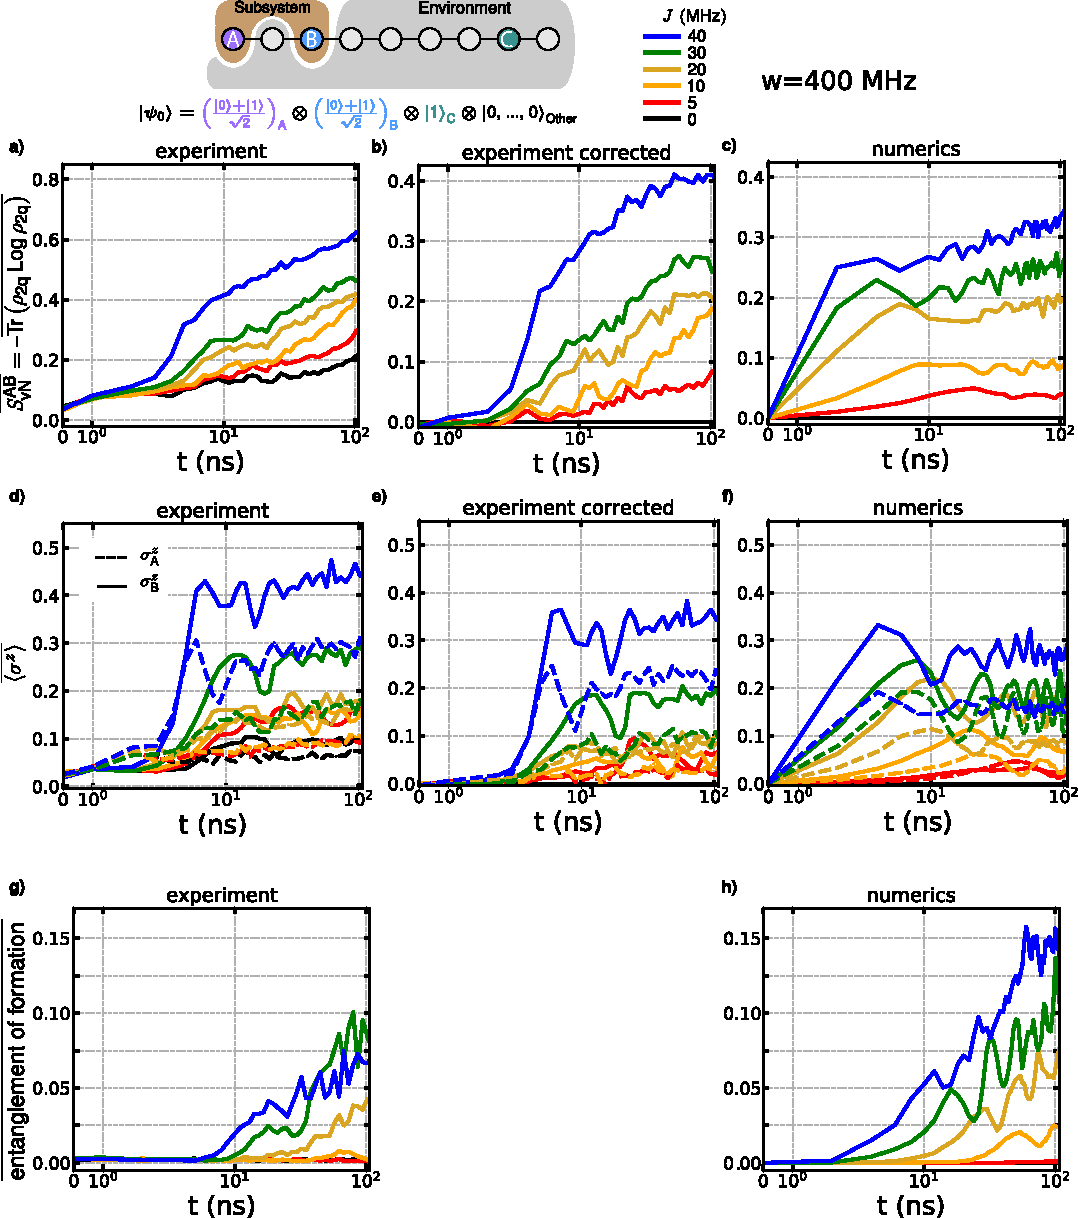
\includegraphics[width=140mm, keepaspectratio]{./PDF/dat_cor_num_superposition_log.pdf}
\caption{Data from Fig.\,S11 plotted on semi-log axes to emphasize scaling.  The disagreement at short times is attributed to the transient respose of the control pulses.}
\end{figure*}

\subsection{Comparison with numerics for bell initial state.}
\begin{figure*}
\centering
\hspace*{10mm}
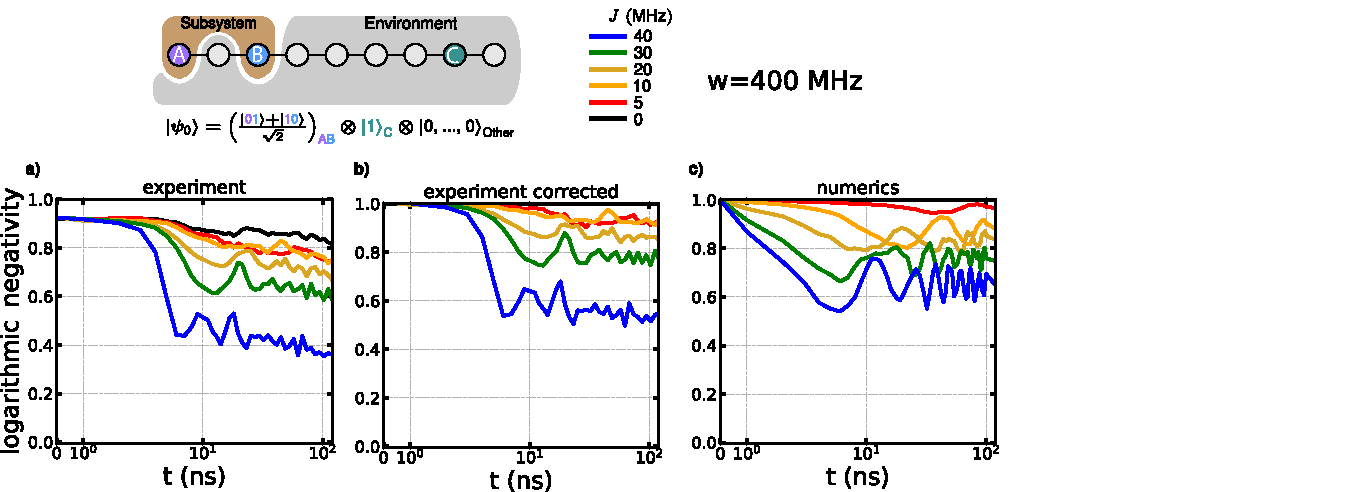
\includegraphics[width=195mm, keepaspectratio]{./PDF/dat_cor_num_bell_log.pdf}
\caption{Data from Fig.\,S12 plotted on semi-log axes to emphasize scaling.  The disagreement at short times is attributed to the transient respose of the control pulses.}
\end{figure*}

\subsection{Long time numerics for superposition initial state.}
\begin{figure*}
\centering
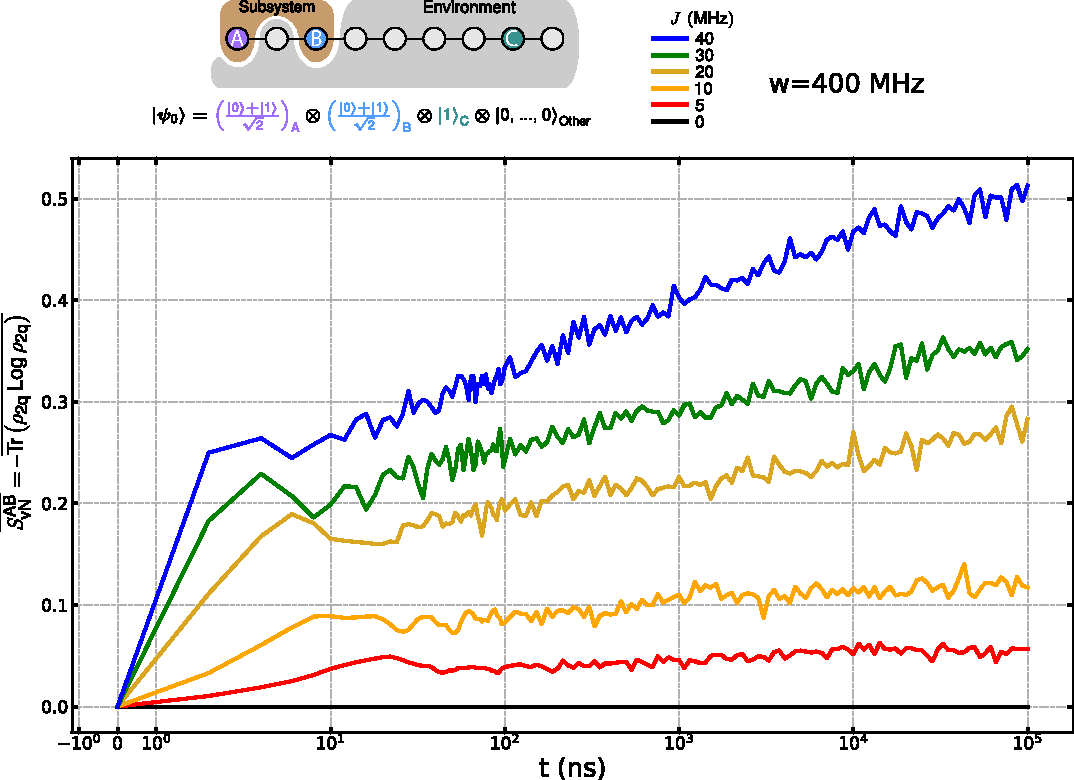
\includegraphics[width=140mm, keepaspectratio]{./PDF/num_svn_long_time.pdf}
\caption{\textbf{Entropy comparison with numerics.}
Numerics to longer times than are accessible in the experiment illustrating the predicted logarithmic growth of entanglement for our system.
}
\end{figure*}

\section{Sensitivity to nonlinearity $U$, Figs.\,S16-S18}
The Hamiltonian parameter $U$ varies weakly as a function of the qubit frequencies and inter-qubit coupling.
$U$ cannot be controlled independently in our system.
Here we provide numerical evidence that the dynamics that we report in the MBL regime are not sensitive to this parameter.
\subsection{Sensitivity of $S_{\text{vN}}^{\text{AB}}$ to nonlinearity $U$}
\begin{figure*}
\centering
\hspace*{20 mm}
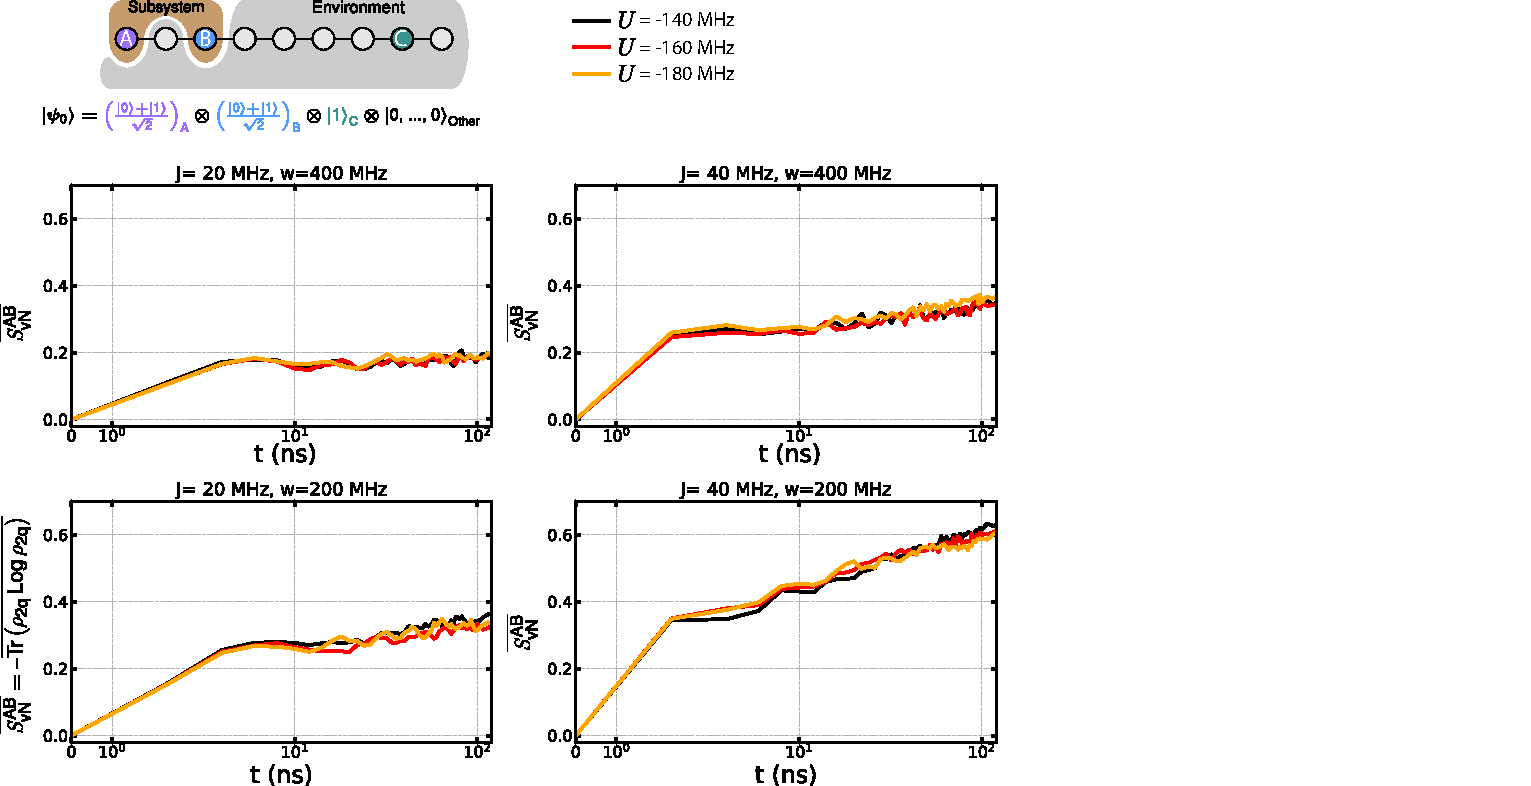
\includegraphics[width=200mm, keepaspectratio]{./PDF/eta_svn.pdf}
\caption{\textbf{Disorder averaged von Neumann entropy vs. $U$ for selected couplings and disorder magnitudes.}  The von Neumann entropy observed in the experiment is predicted to be insensitive to the precise value of $U$.}
\end{figure*}

\subsection{Sensitivity of entanglement of formation to nonlinearity $U$}
\begin{figure*}[tbh]
\centering
\hspace*{20 mm}
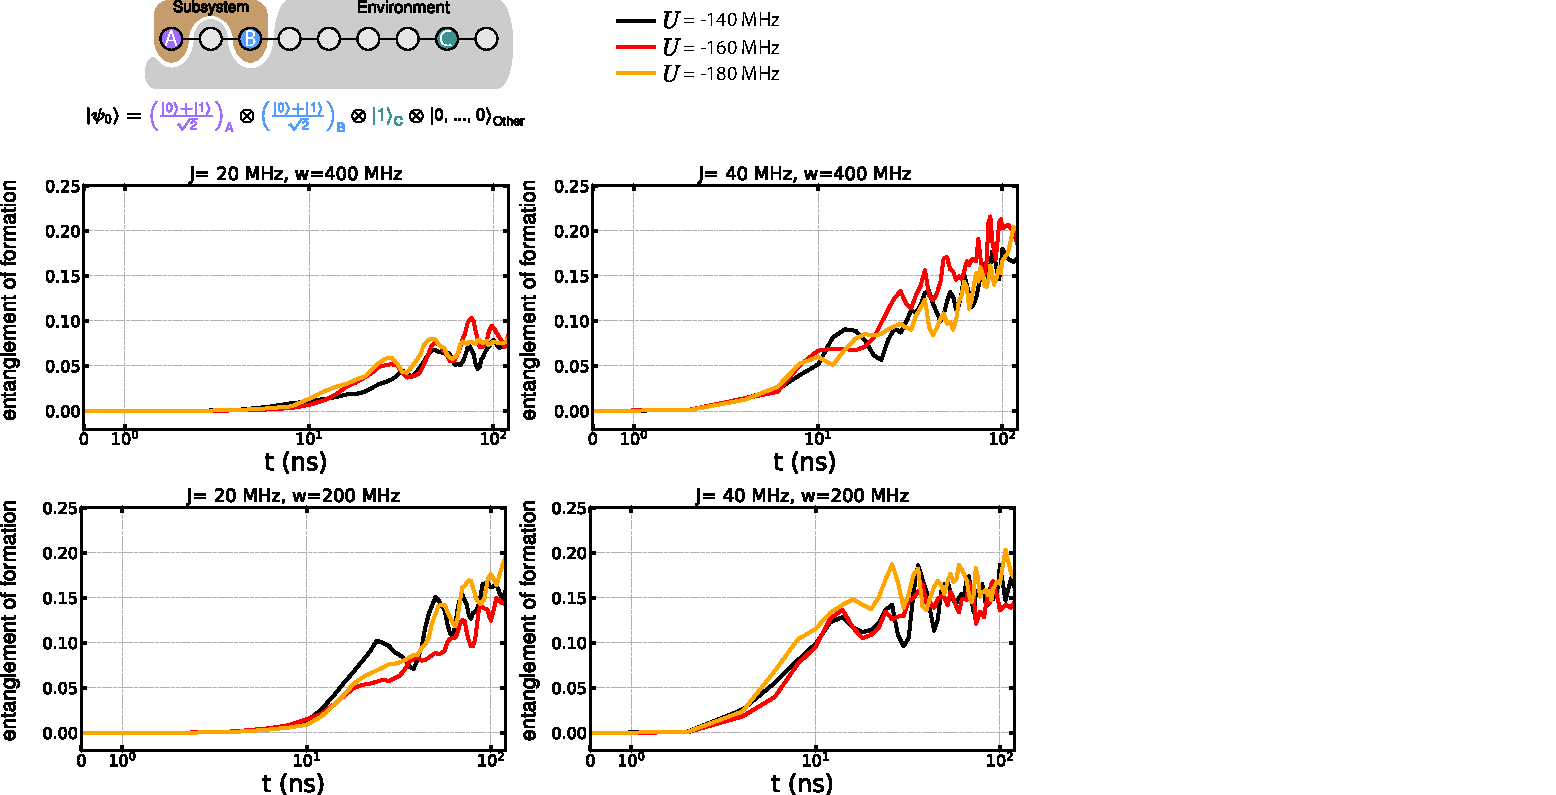
\includegraphics[width=200mm, keepaspectratio]{./PDF/eta_eof.pdf}
\caption{
\textbf{Disorder averaged entanglement of formation vs. $U$ for selected couplings and disorder magnitudes.}
The entanglement of formation observed in the experiment is predicted to be insensitive to the precise value of $U$.}
\end{figure*}

\subsection{Sensitivity of $\sigma^z$ to nonlinearity $U$}
\begin{figure*}[h]
\centering
\hspace*{20 mm}
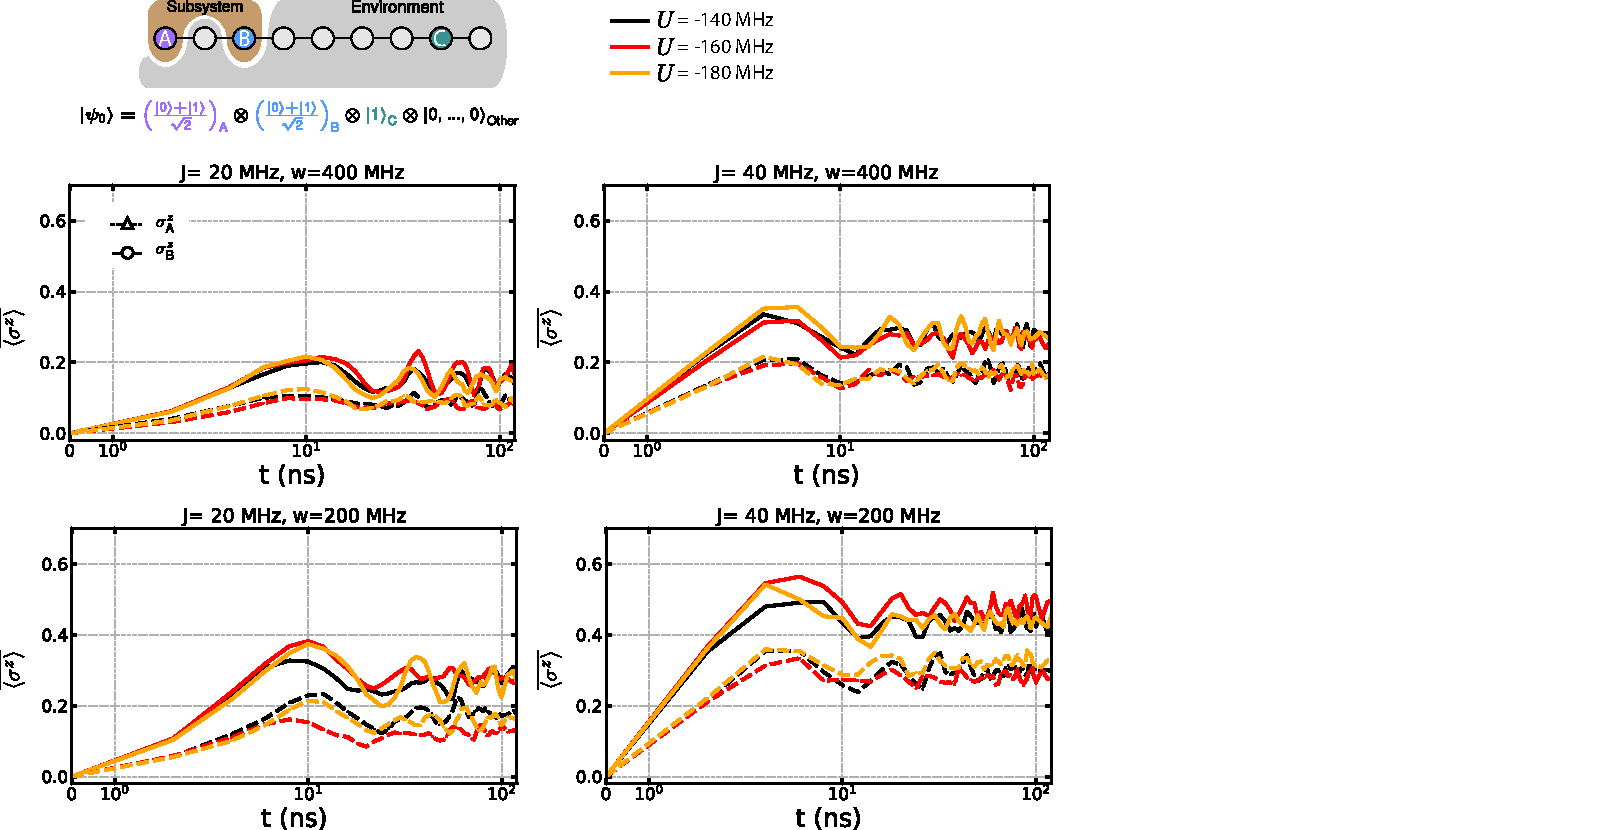
\includegraphics[width=200mm, keepaspectratio]{./PDF/eta_ziiz.pdf}
\caption{\textbf{$\overline{\left< \sigma^z \right>}$ vs. $U$ for selected couplings and disorder magnitudes.}
The onsite population observed in the experiment is predicted to be insensitive to the precise value of $U$.}

\end{figure*}

\section{Extended data for 1D qubit array, Fig.\,S19}
\subsection{Distillable entanglement in MBL and diffusive regimes}
\begin{figure*}[h]
\centering
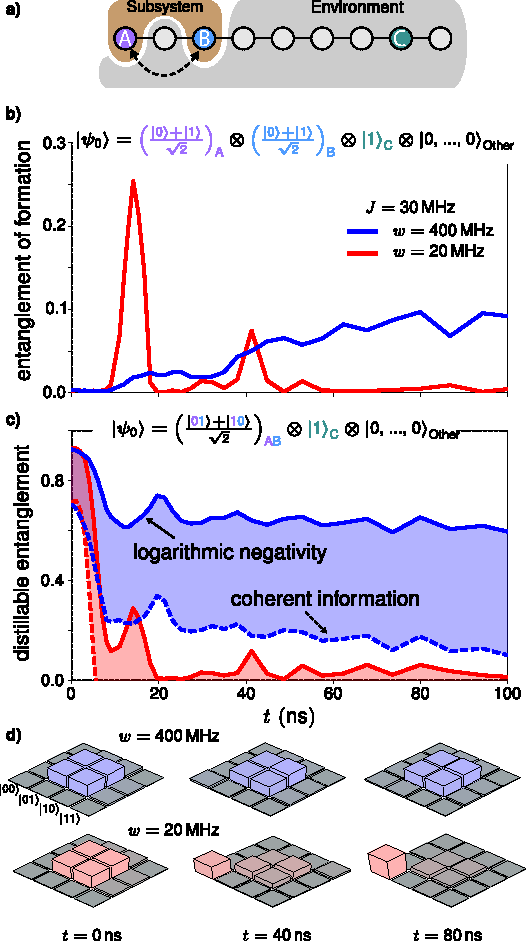
\includegraphics[width=89mm, keepaspectratio]{./PDF/f6_190716_1129a.pdf}
\caption{\textbf{Entanglement of formation and distillable entanglement in MBL and diffusive regimes}
        \textbf{(a)} Schematic diagram emphasizing our focus on the entanglement between qubits A and B which are embedded in an environment.
        \textbf{(b)} To observe the development of entanglement between sites A and B the sub-system is initialized in a product of single qubit superposition states and the entanglement of formation of the two qubit density matrix is extracted.
        \textbf{(c)} We demonstrate the capability of the MBL phase to preserve entanglement initializing the sub-system into a maximally entangled Bell pair and observing the decay of quantum correlations.
        We extract the logarithmic negativity and coherent information from measurements of the two-qubit sub-system density matrix.
        These provide, respectively, upper and lower bounds on the distillable entanglement within the sub-system.
        \textbf{(d)} Representative density matrices from single disorder instances contained in \textbf{(c)} at high and low disorder.
        }

\end{figure*}

In a 1D system we investigate the formation and preservation of entanglement between two qubits A and B that are embedded in a many-body localized environment as illustrated in Fig.\,S19\,(a) and contrast this behavior with a system in the diffusive regime.
%From the quantum information point of view it is interesting to know how entanglement develops between specified sub-system qubits.
%We therefore emphasize measures that describe the entanglement between parts of the sub-system in Fig. 6 as illustrated in panel (a).
The entanglement of formation quantifies the amount of entanglement directly between qubits A and B that would be required to produce the observed two-qubit mixed state density matrix.%\autocite{Wootters1998}
In panel (b), we initialize the sub-system into an unentangled product state of single qubit superpositions and observe the development of entanglement between our sub-system qubits.
At high disorder, associated with the localized phase, entanglement grows continuously between the spatially separated sites.
At low disorder, corresponding with the ergodic phase, we observe brief intervals of significant entanglement as the excitations delocalize across the full 9 qubit system.
However, this behavior is quickly damped as the excitations are absorbed by environmental qubits, as the full 9-qubit system thermalizes.

%While the results discussed thus far show interaction effects between the LIOMs, it is also a major prospect to demonstrate the preservation of quantum information in such a system.
Systems in the MBL and diffusive regimes also differ in their ability to retain correlation between their constituent parts.  This is illustrated in Fig.\,S19\,(B) where we prepare a distant Bell state between the first and the third qubit and study the entanglement dynamics.
While dephasing between LIOMs will ultimately destroy the entanglement, it will only due so on exponentially long times due to the localization.
Crucially, the subsystem is in a mixed state, because it is coupling to the other 7 qubits of our device.
We therefore characterize the entanglement of the 2-body mixed density matrix $\rho_{2q} \left( t \right)$ using an operational entanglement measure.
In particular, we focus on the distillable entanglement, i.e., the entanglement which can be extracted from the mixed density matrix, that is upper bounded by logarithmic negativity entropy and lower bounded by the coherent information entropy.
These bounds are shown in panel (c). For weak disorder (red), the prepared quantum information is immediately lost because the quantum dynamics entangles the subsystem with its environment and a featureless high temperature state is attained locally.
%
This behavior can also be understood in terms of the monogamy of entanglement.\autocite{Wootters2000}
Although the two qubit subsystem is initially prepared in a maximally entangled state the degree of quantum correlation between subsystem sites decreases as the subsystem exchanges information with the environment and entangles with it.
This monogamic principle also explains the damping of the peak in the low disorder data of panel (b).
%
However, for strong disorder (blue) the distillable entanglement is sizable over long times, and hence the density matrix can be used as quantum resource.
This is exemplified in panel (d) which shows the tomographic reconstruction of the two qubit density matrix for a single disorder instance as it evolves in time.
These results show that a many-body localized system can efficiently retain quantum information over long time scales.

\section{Extended data for 2D qubit arrays, Fig.\,S20}
\subsection{Onsite population for 2D qubit arrays}
\begin{figure*}[tbh]
\centering
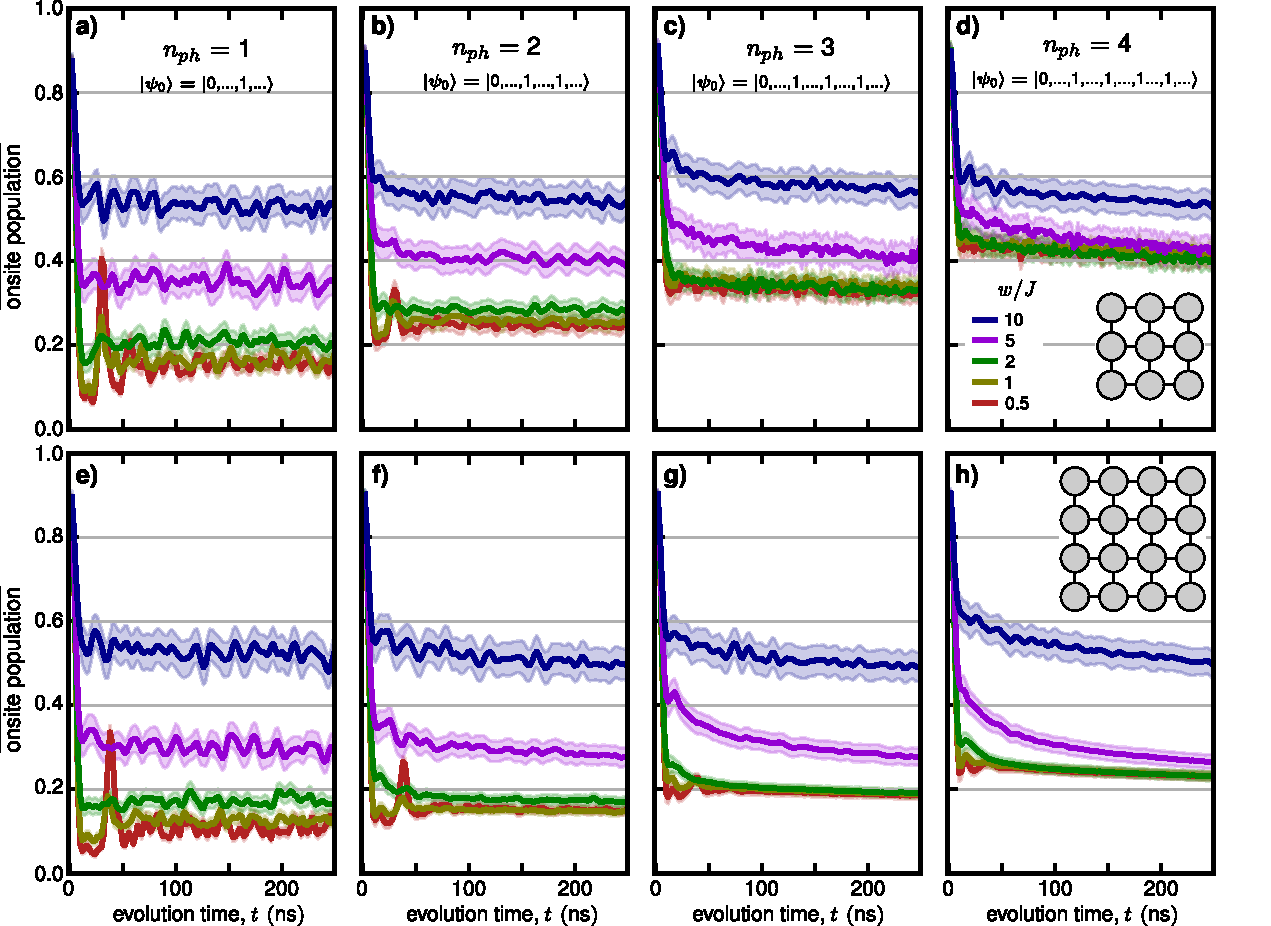
\includegraphics[width=175mm, keepaspectratio]{./PDF/population_2d_190915_1018a.pdf}
\caption{\textbf{Extended data for onsite population of 2D arrays.}
\textbf{(a-d)} Onsite population for $n_{ph} = 1,2,3,4$ on a 3x3 array of qubits.
\textbf{(e-h)} Onsite population for $n_{ph} = 1,2,3,4$ on a 4x4 array of qubits.}
\end{figure*}

In Fig.\,S20, we show extended data for the onsite population for 2D geometries, for $n_{ph}=1,2,3,4$.  The initial location of the excitations was randomized between runs but the observation site was always one of the initially excited qubits.  Similar to the 1D geometries, with sufficient disorder the onsite population takes a non-thermal stationary value and is consistent with many-body localization.  In the 2D geometries the onsite population consistent with thermalization at higher disorders when there are more photons in the system (greater $n_{ph}$), as in the 1D case.

